% \documentclass[aspectratio=169]{beamer}
\documentclass[aspectratio=169, notes]{beamer}
\usepackage[utf8]{inputenc}
\usepackage[inline]{enumitem}
\usepackage{pdfpages}
\usepackage{listings}
\usepackage{subcaption}
\usepackage{wasysym}
\usepackage[export]{adjustbox}[2011/08/13]
\usetheme{cern}

\addtobeamertemplate{note page}{}{\thispdfpagelabel{notes:\insertframenumber}}

\newcommand\FourQuad[4]{%
    \begin{minipage}[b][.35\textheight][t]{.47\textwidth}#1\end{minipage}\hfill%
    \begin{minipage}[b][.35\textheight][t]{.47\textwidth}#2\end{minipage}\\[0.5em]
    \begin{minipage}[b][.35\textheight][t]{.47\textwidth}#3\end{minipage}\hfill
    \begin{minipage}[b][.35\textheight][t]{.47\textwidth}#4\end{minipage}%
}

\newcommand{\btVFill}{\vskip0pt plus 1filll}

% fix tilde
% \newcommand{\propertilde}{\raise.17ex\hbox{$\scriptstyle\mathtt{\sim}$}}

% \setbeameroption{show notes on second screen=right}

%The CERN logo is legally protected. Please visit http://cern.ch/copyright for
%information on the terms of use of CERN content, including the CERN logo.

% The optional `\author` command defines the author and is displayed in the
%slide produced by the `\titlepage` command.
\author{Corné Lukken \& Animesh Trivedi}

% The optional `\title` command defines the title and is displayed in the slide
%produced by the `\titlepage` command.
\title{OpenCSD, simple and intuitive computational storage emulation with QEMU and eBPF}

% The optional `\subtitle` command will add a smaller title below the main one,
%and will not be displayed in any of the slides' footer.
% \subtitle{A SPDK compared to lightnvm story}

% The optional `\date` command will display a custom free text date on the all
%of the slides' footer. If omitted today's date will be used.
%\date{Monday, 1st January 2018}

% ------------------------------------------------------------------------%
% Proper Python Syntax Highlighting                                       %
% Author: redmode
% https://tex.stackexchange.com/questions/83882/how-to-highlight-python   %
% -syntax-in-latex-listings-lstinputlistings-command#83883                %
% ----------------------------------------------------------------------- %

% Default fixed font does not support bold face
\DeclareFixedFont{\ttb}{T1}{txtt}{bx}{n}{6} % for bold
\DeclareFixedFont{\ttm}{T1}{txtt}{m}{n}{6}  % for normal

% Custom colors
\definecolor{deepblue}{rgb}{0,0,0.5}
\definecolor{deepred}{rgb}{0.6,0,0}
\definecolor{deepgreen}{rgb}{0,0.5,0}

% Python style for highlighting
\newcommand\pythonstyle{
	\lstset{
		language=Python,
		basicstyle=\ttm,
		showstringspaces=false,
		tabsize=2,
		aboveskip=0.1cm,
		belowskip=0.1cm,
		otherkeywords={self},             % Add keywords here
		keywordstyle=\ttb\color{deepblue},
		emph={MyClass,__init__},          % Custom highlighting
		emphstyle=\ttb\color{deepred},    % Custom highlighting style
		stringstyle=\color{deepgreen},
		frame=tb,                          % Any extra options here
		prebreak=\textbackslash,
		linewidth=7.00cm,
		breaklines=true,
	}
}

% Python environment
\lstnewenvironment{python}[1][] {
	\pythonstyle\lstset{#1}
}{}

% Python for inline
\newcommand\pythoninline[1]{{\pythonstyle\lstinline!#1!}}

% Python for external file
\newcommand\pythonexternal[2][]{{\pythonstyle\lstinputlisting[#1]{#2}}}

\newcommand\pythonfullstyle{
	\lstset{
		language=Python,
		basicstyle=\ttm,
		showstringspaces=false,
		tabsize=2,
		aboveskip=0.1cm,
		belowskip=0.1cm,
		otherkeywords={self},             % Add keywords here
		keywordstyle=\ttb\color{deepblue},
		emph={MyClass,__init__},          % Custom highlighting
		emphstyle=\ttb\color{deepred},    % Custom highlighting style
		stringstyle=\color{deepgreen},
		frame=tb,                          % Any extra options here
		prebreak=\textbackslash,
		linewidth=11.00cm,
		breaklines=true,
	}
}

% Python environment
\lstnewenvironment{pythonfull}[1][] {
	\pythonfullstyle\lstset{#1}
}{}

% Python for inline
\newcommand\pythonfullinline[1]{{\pythonfullstyle\lstinline!#1!}}

% Python for external file
\newcommand\pythonfullexternal[2][]{{\pythonfullstyle\lstinputlisting[#1]{#2}}}

% ----------------------------------------------------------------------- %

% Bash style for highlighting
\newcommand\bashstyle{
	\lstset{
		language=Bash,
		basicstyle=\ttm,
		showstringspaces=false,
		tabsize=2,
		%commentstyle=itshape,
		aboveskip=0.1cm,
		belowskip=0.1cm,
		prebreak=\textbackslash,
		extendedchars=true,
		mathescape=false,
		% literate= {\$}{{\textcolor{blue}{\$}}}1 {&}{{\textcolor{blue}{\&}}}1 {/n}{{\textcolor{green}{\textbackslash n}}}1,
		linewidth=11cm,
		breaklines=true
	}
}

% Bash environment
\lstnewenvironment{bash}[1][] {
	\bashstyle\lstset{#1}
}{}

% Bash for inline
\newcommand\bashinline[1]{{\bashstyle\lstinline!#1!}}

% Bash for external file
\newcommand\bashexternal[2][]{{\bashstyle\lstinputlisting[#1]{#2}}}

% Python style for highlighting
\newcommand\cstyle{
	\lstset{
		language=c,
		basicstyle=\ttm,
		showstringspaces=false,
		tabsize=4,
		aboveskip=0.2cm,
		belowskip=0.2cm,
		otherkeywords={self},             % Add keywords here
		emph={MyClass,__init__},          % Custom highlighting
		keywordstyle=\ttb\color{deepblue},
		emphstyle=\ttb\color{deepred},    % Custom highlighting style
		stringstyle=\ttm\color{deepgreen},
%		identifierstyle=\ttm,
%		commentstyle=\ttm,
%		numberstyle=\ttm,
%		indexstyle=\ttm,
%		directivestyle=\ttm,
		frame=tb,                          % Any extra options here
		prebreak=\textbackslash,
		linewidth=5cm,
		breaklines=true,
	}
}

% Python environment
\lstnewenvironment{clist}[1][] {
	\cstyle\lstset{#1}
}{}

% Python for inline
\newcommand\cinline[1]{{\cstyle\lstinline!#1!}}

% Python for external file
\newcommand\cexternal[2][]{{\cstyle\lstinputlisting[#1]{#2}}}

\begin{document}

% This presentation is about OpenCSD and FluffleFS a open-source, open-data
% simulation platform with multi-user tenant filesystem for Compational Storage
% Devices. While this work solves several open research questions we will only
% be able to highlight one today. Particularly, compatability with user
% compiled code, safety and synchronization are not covered. First we
% demonstrate why we need Computational storage in the first place.

\frame{\titlepage}
\note{
    30s - 0.5
    \begin{itemize}
        \item Emulating computational storage with QEMU and eBPF
        \item QEMU is used to simplify setup but not strictly necessary
    \end{itemize}
}

\begin{frame}{Index}
    \begin{columns}
        \begin{column}{0.6\textwidth}
            \begin{itemize}
                \item Who am I
                \item What is Computational Storage
                \begin{itemize}
                    \item \footnotesize Why do we Need it
                    \item \footnotesize State of Current Prototypes
                \end{itemize}
                \item OpenCSD \& FluffleFS
                \begin{itemize}
                    \item \footnotesize Key Design Aspects
                    \item \footnotesize Component Breakdown
                    \item \footnotesize Shannon Entropy Demo
                    \item \footnotesize Operating Principle Details
                    \item \footnotesize Limitations and Considerations
                \end{itemize}
                \item Future Work
            \end{itemize}
        \end{column}
        \begin{column}{0.4\textwidth}
        \end{column}
    \end{columns}
\end{frame}
\note{
    30s - 1.0
    \begin{itemize}
        \item What we will talk about today
        \item Some introduction
        \item Most probably unfamiliar with computational storage
        \item Show how to install and run OpenCSD and FluffleFS
        \item Show some code examples and a demo
        \item Describe the API and how to create your own computational
              storage kernels
    \end{itemize}
}

\begin{frame}{Who am I}
    \begin{itemize}
        \item Corne Lukken - Dantali0n
        \item Parallel \& Distributed Systems
        \item Academia
        \begin{itemize}
            \item \footnotesize Bachelor Software Engineering (AUAS)
            \item \footnotesize Master Computer Science (VU / UvA)
        \end{itemize}
        \item Experience
        \begin{itemize}
            \item \footnotesize Health Technology @ AUAS
            \item \footnotesize Openstack @ CERN
            \item \footnotesize Computational Storage @ VU
            \item \footnotesize SCADA @ ASTRON
        \end{itemize}
    \end{itemize}
\end{frame}
\note{
    30s - 1.5
    \begin{itemize}
        \item 12 years of academia including an associate, bachelor and master degree
        \item Health Technology - Outdoor Navigation for visually impaired
        \item Openstack - Cloud Optimization by live migration
        \item Computational Storage - This talk
        \item SCADA - LOFAR 2 station software
    \end{itemize}
}

\begin{frame}{Why do we need it}
    \begin{columns}
        \begin{column}{0.3\textwidth}
%             \begin{itemize}
%                 \item test
%             \end{itemize}
        \end{column}
        \begin{column}{0.7\textwidth}
            \begingroup
            \small
            \begin{figure}
                \centering
                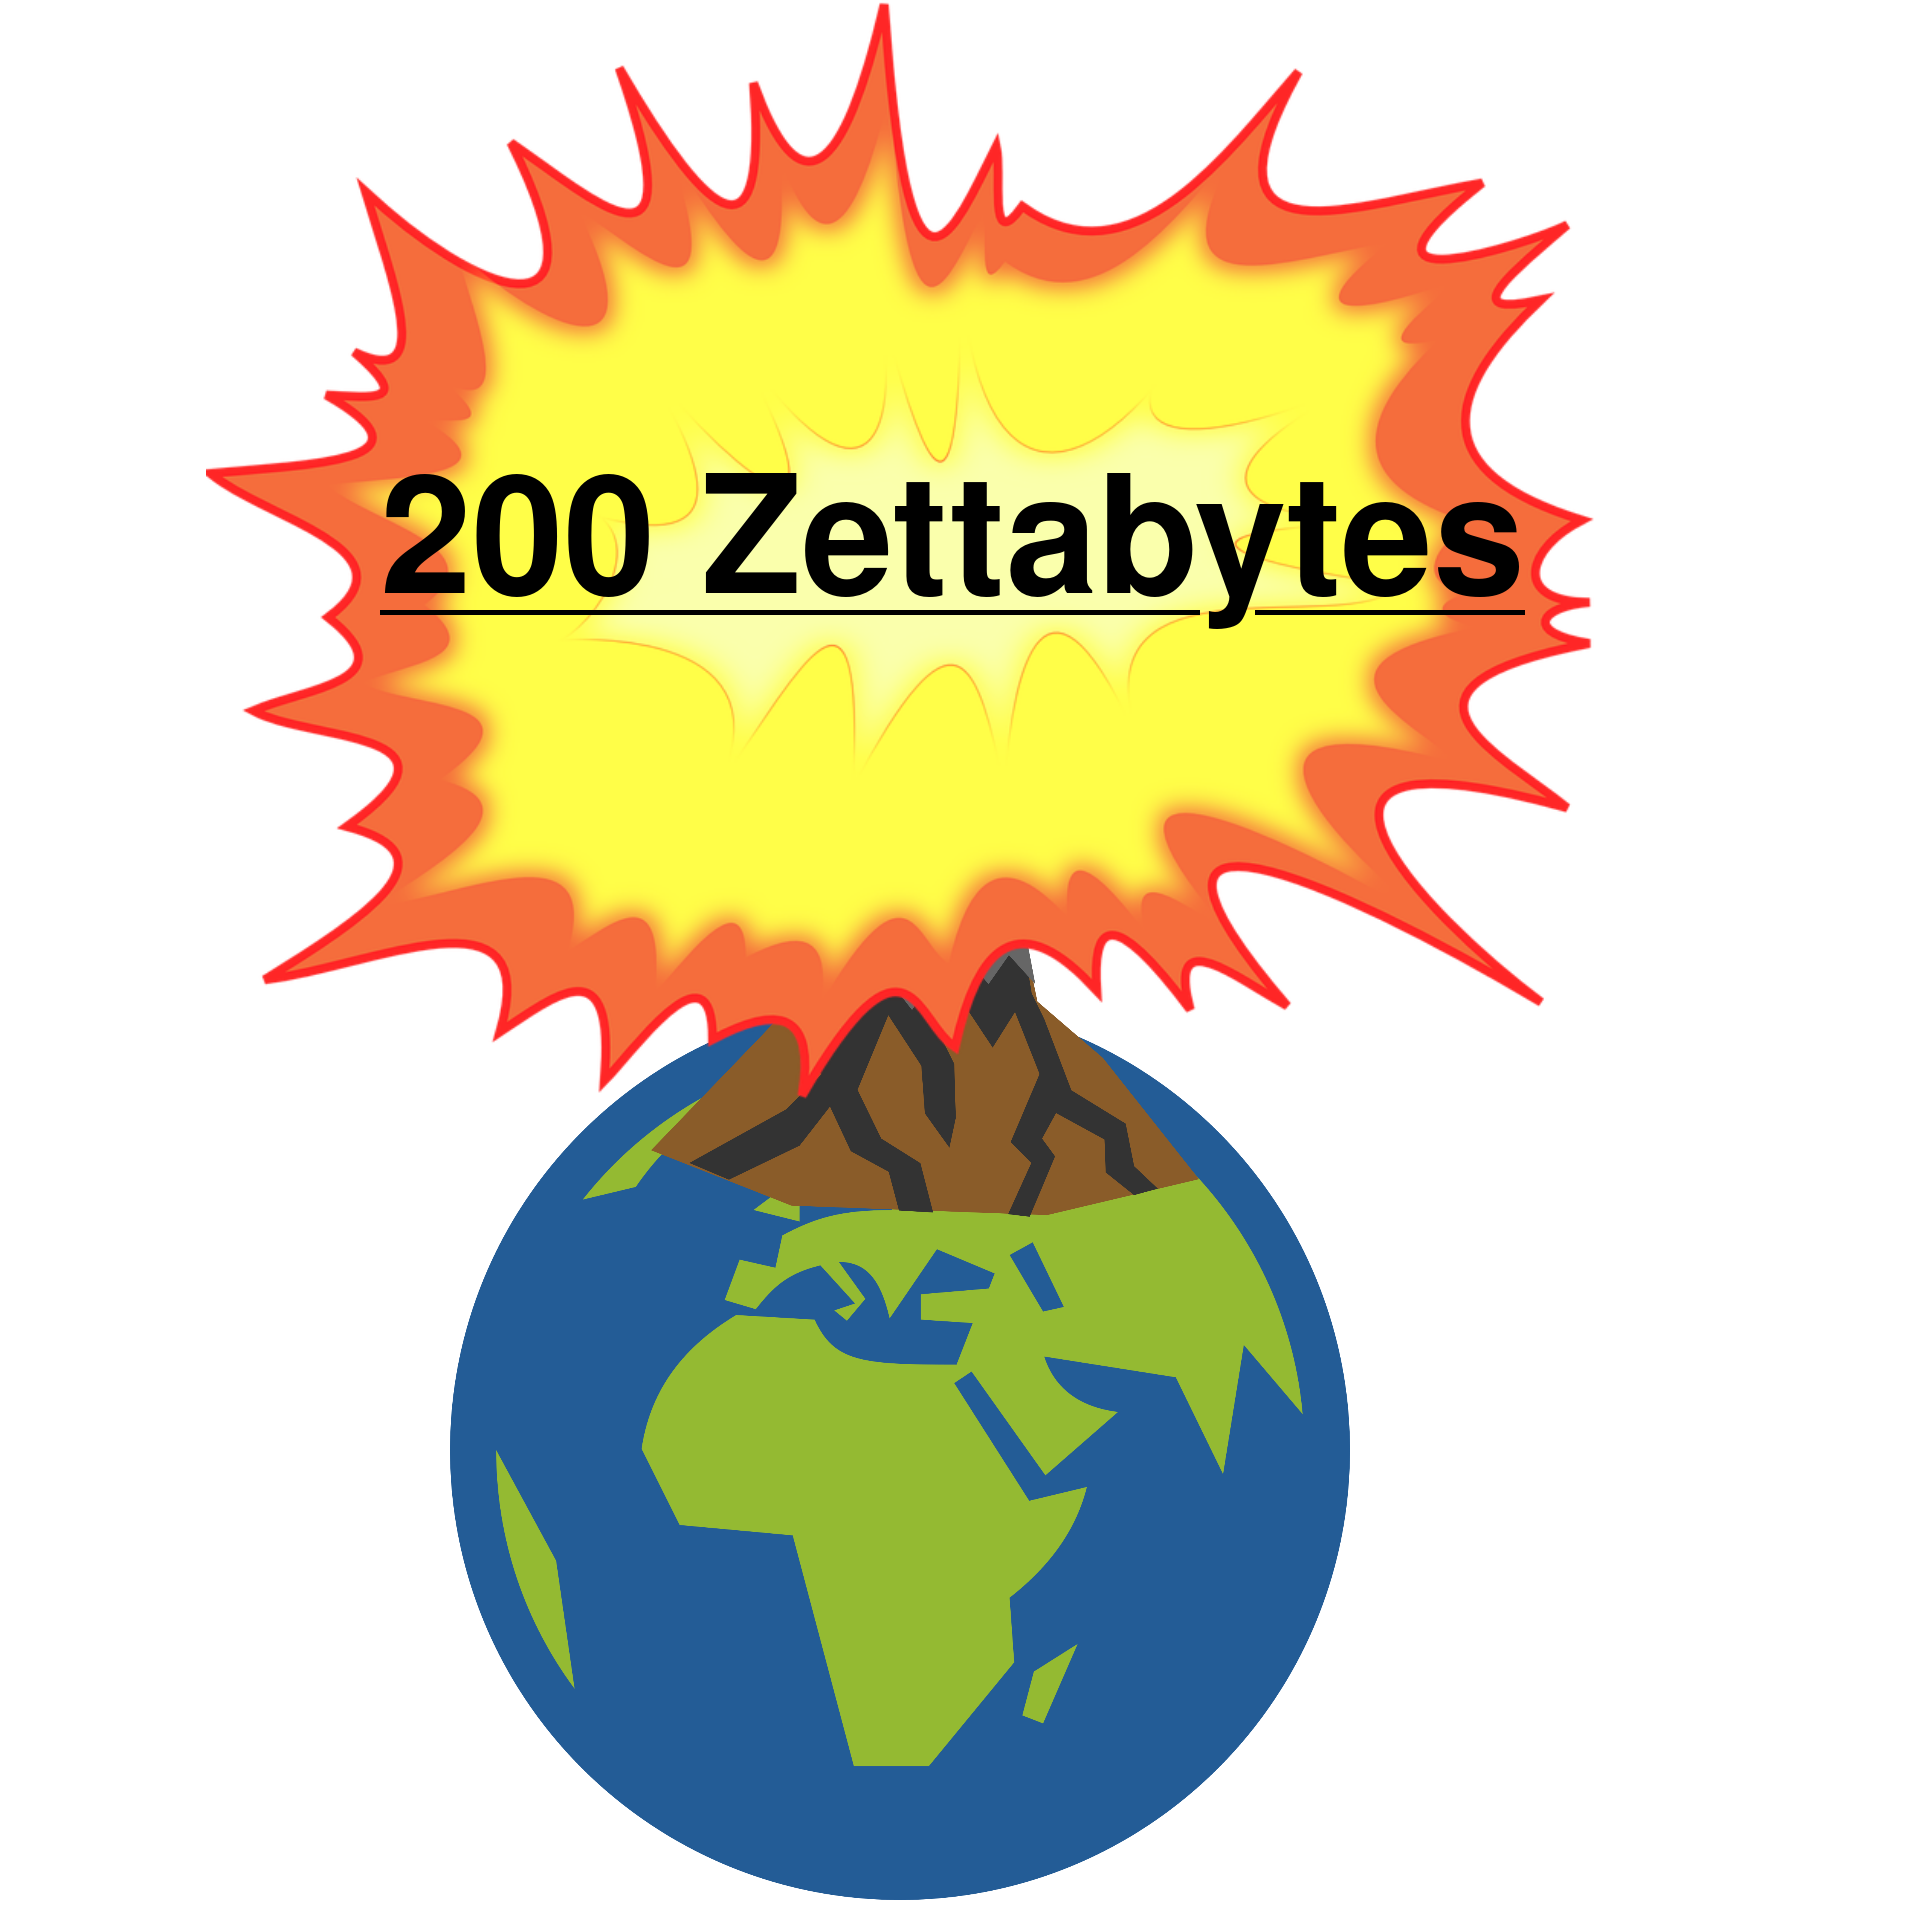
\includegraphics[width=0.9\textwidth]{resources/images/data-problem.png}
            \end{figure}
            \endgroup
        \end{column}
    \end{columns}
\end{frame}
\note{
    1m - 2.5
    \begin{itemize}
        \item We life in a data-driven society, a world exploding data.
        \item So much data that we are expected to store 200 Zettabytes of data
              in total by 2050.
        \item Such high data capacity and throughput requirements pose
              significant challenges to existing and future technologies.
    \end{itemize}
}

% page 2
\begin{frame}{Why do we need it}
    \begin{columns}
        \begin{column}{0.3\textwidth}
            \footnotesize
            \begin{itemize}
            	\item Von Neumann architecture
            	\item Memory bottlenecks
            	\item Interconnect bottlenecks
            	\item Energy efficiency
            \end{itemize}
        \end{column}
        \begin{column}{0.7\textwidth}
            \begingroup
            \small
            \begin{figure}
                \centering
                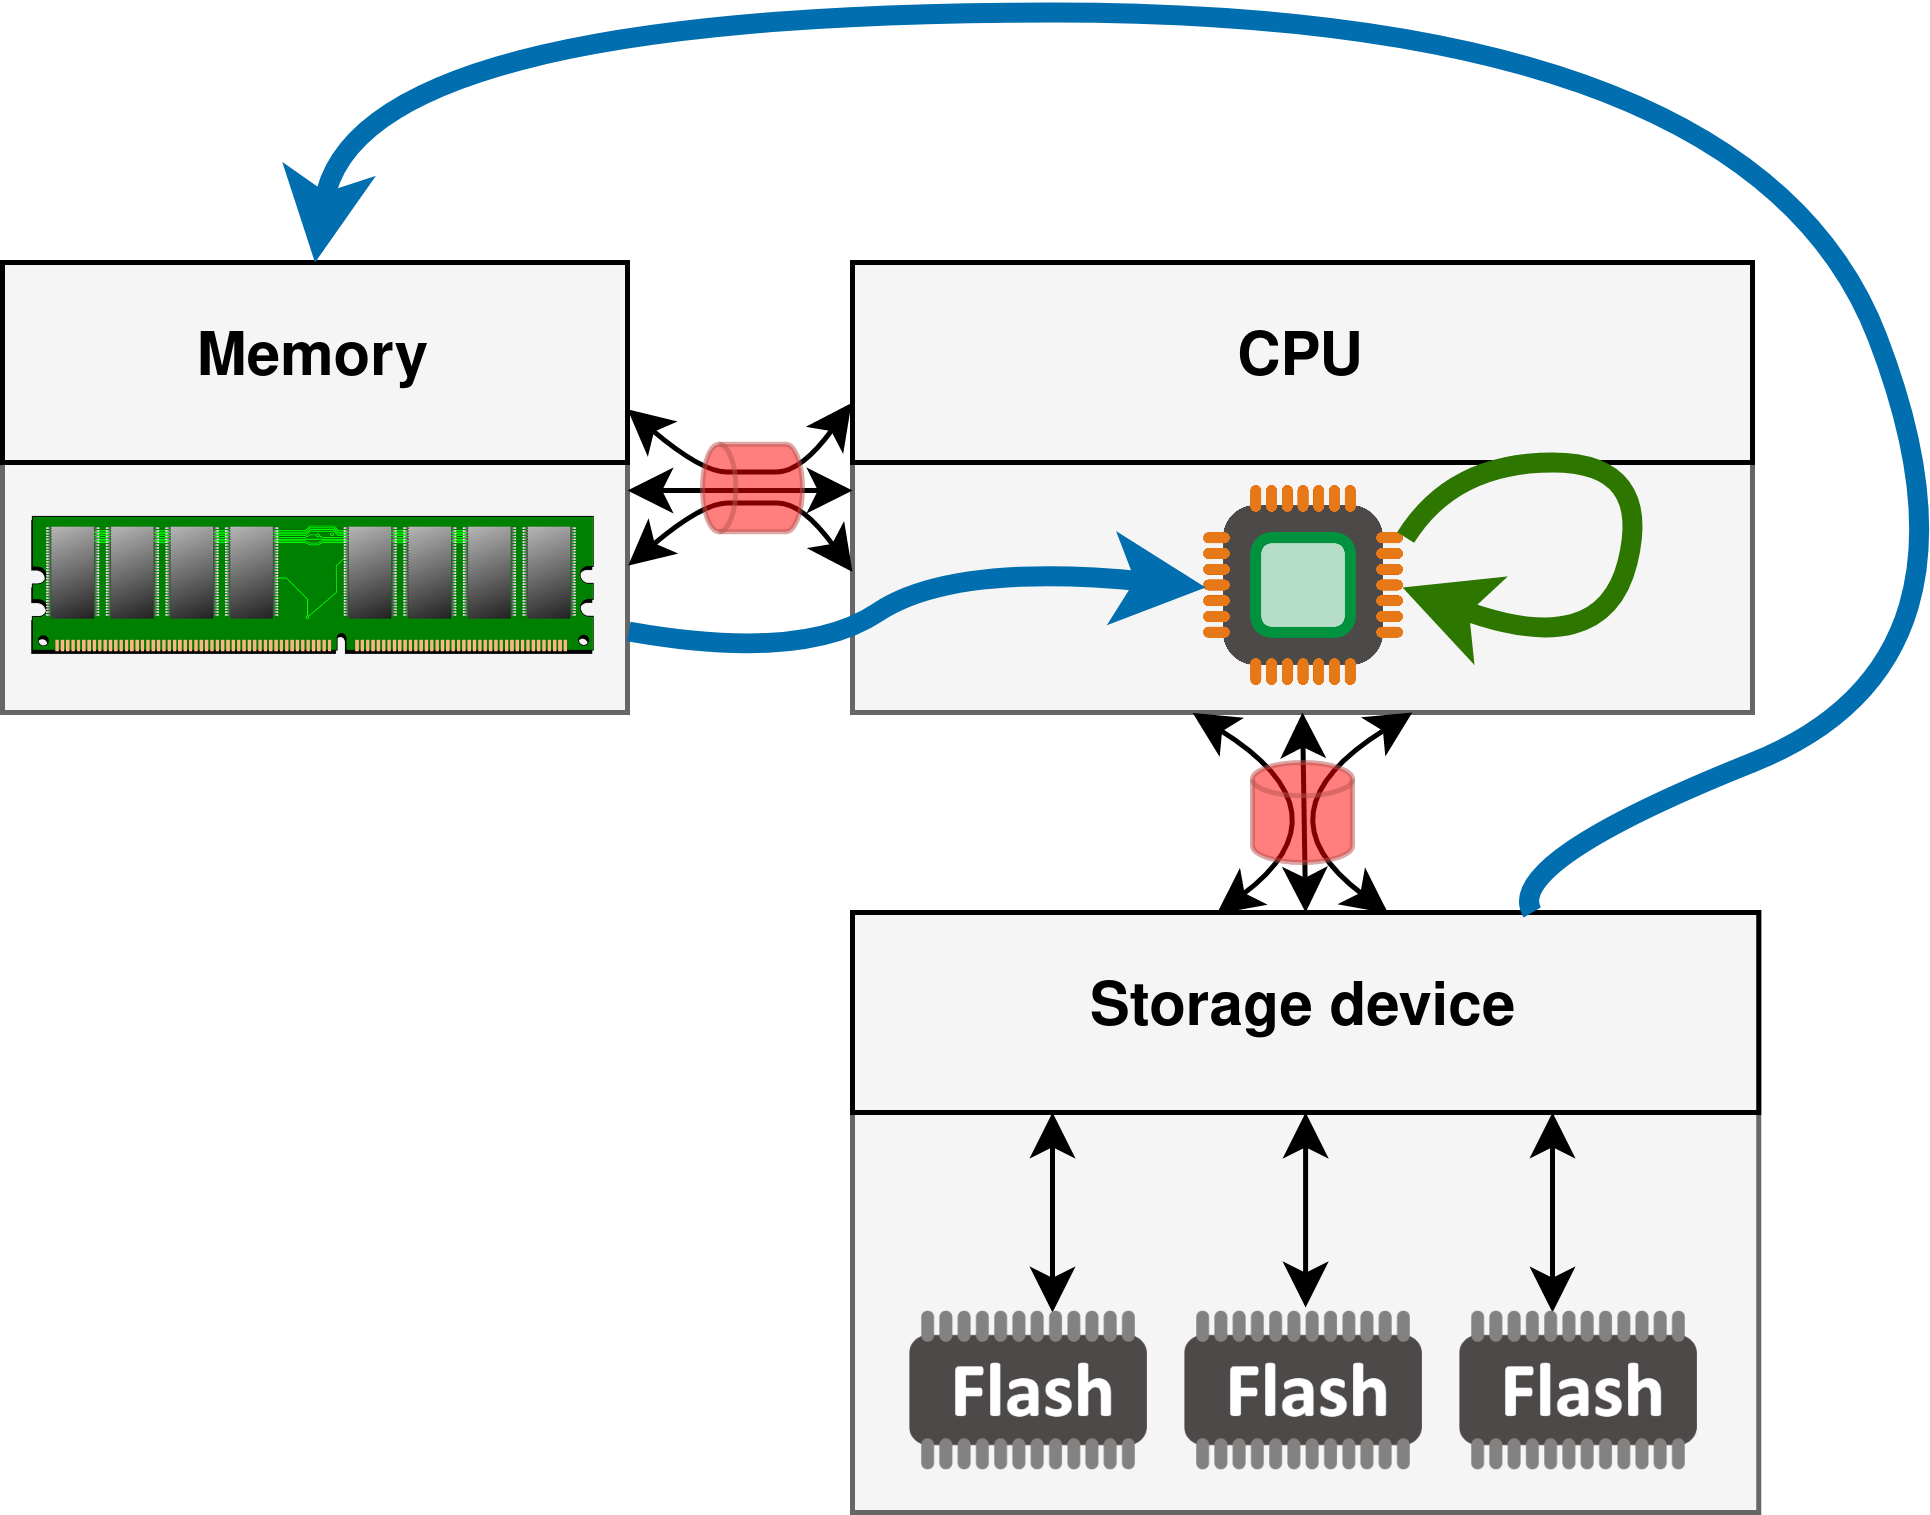
\includegraphics[width=0.7\textwidth]{resources/images/bottleneck.png}
            \end{figure}
            \endgroup
        \end{column}
    \end{columns}
\end{frame}
\note{
    1m - 3.5
    \begin{itemize}
        \item Von Neumann architecture causes most prominent bottleneck
        \item All data needs to be moved to main system memory prior to CPU
              processing.
        \item Prevents processor from directly operating on data.
        \item Memory controller, PCIe root complex, other interconnects and
              networks often have lower bandwidth then SSD storage arrays found
              in enterprise storage servers.
        \item The cost of additional memory and CPU as well as rackspace is
              significant compared to the cost of additional SSD storage.
    \end{itemize}
}

\begin{frame}{Why do we need it}
    \begin{columns}
        \begin{column}{0.3\textwidth}
            \footnotesize
            \begin{itemize}
                \item 4.5x bandwidth gap with 64 SSD storage server (2021)
                \item Flash chip bandwidth under NDA
                \item PCIe p2p-dma \footnotemark[1]
            \end{itemize}
        \end{column}
        \begin{column}{0.7\textwidth}
            \begingroup
            \small
            \begin{figure}
                \centering
                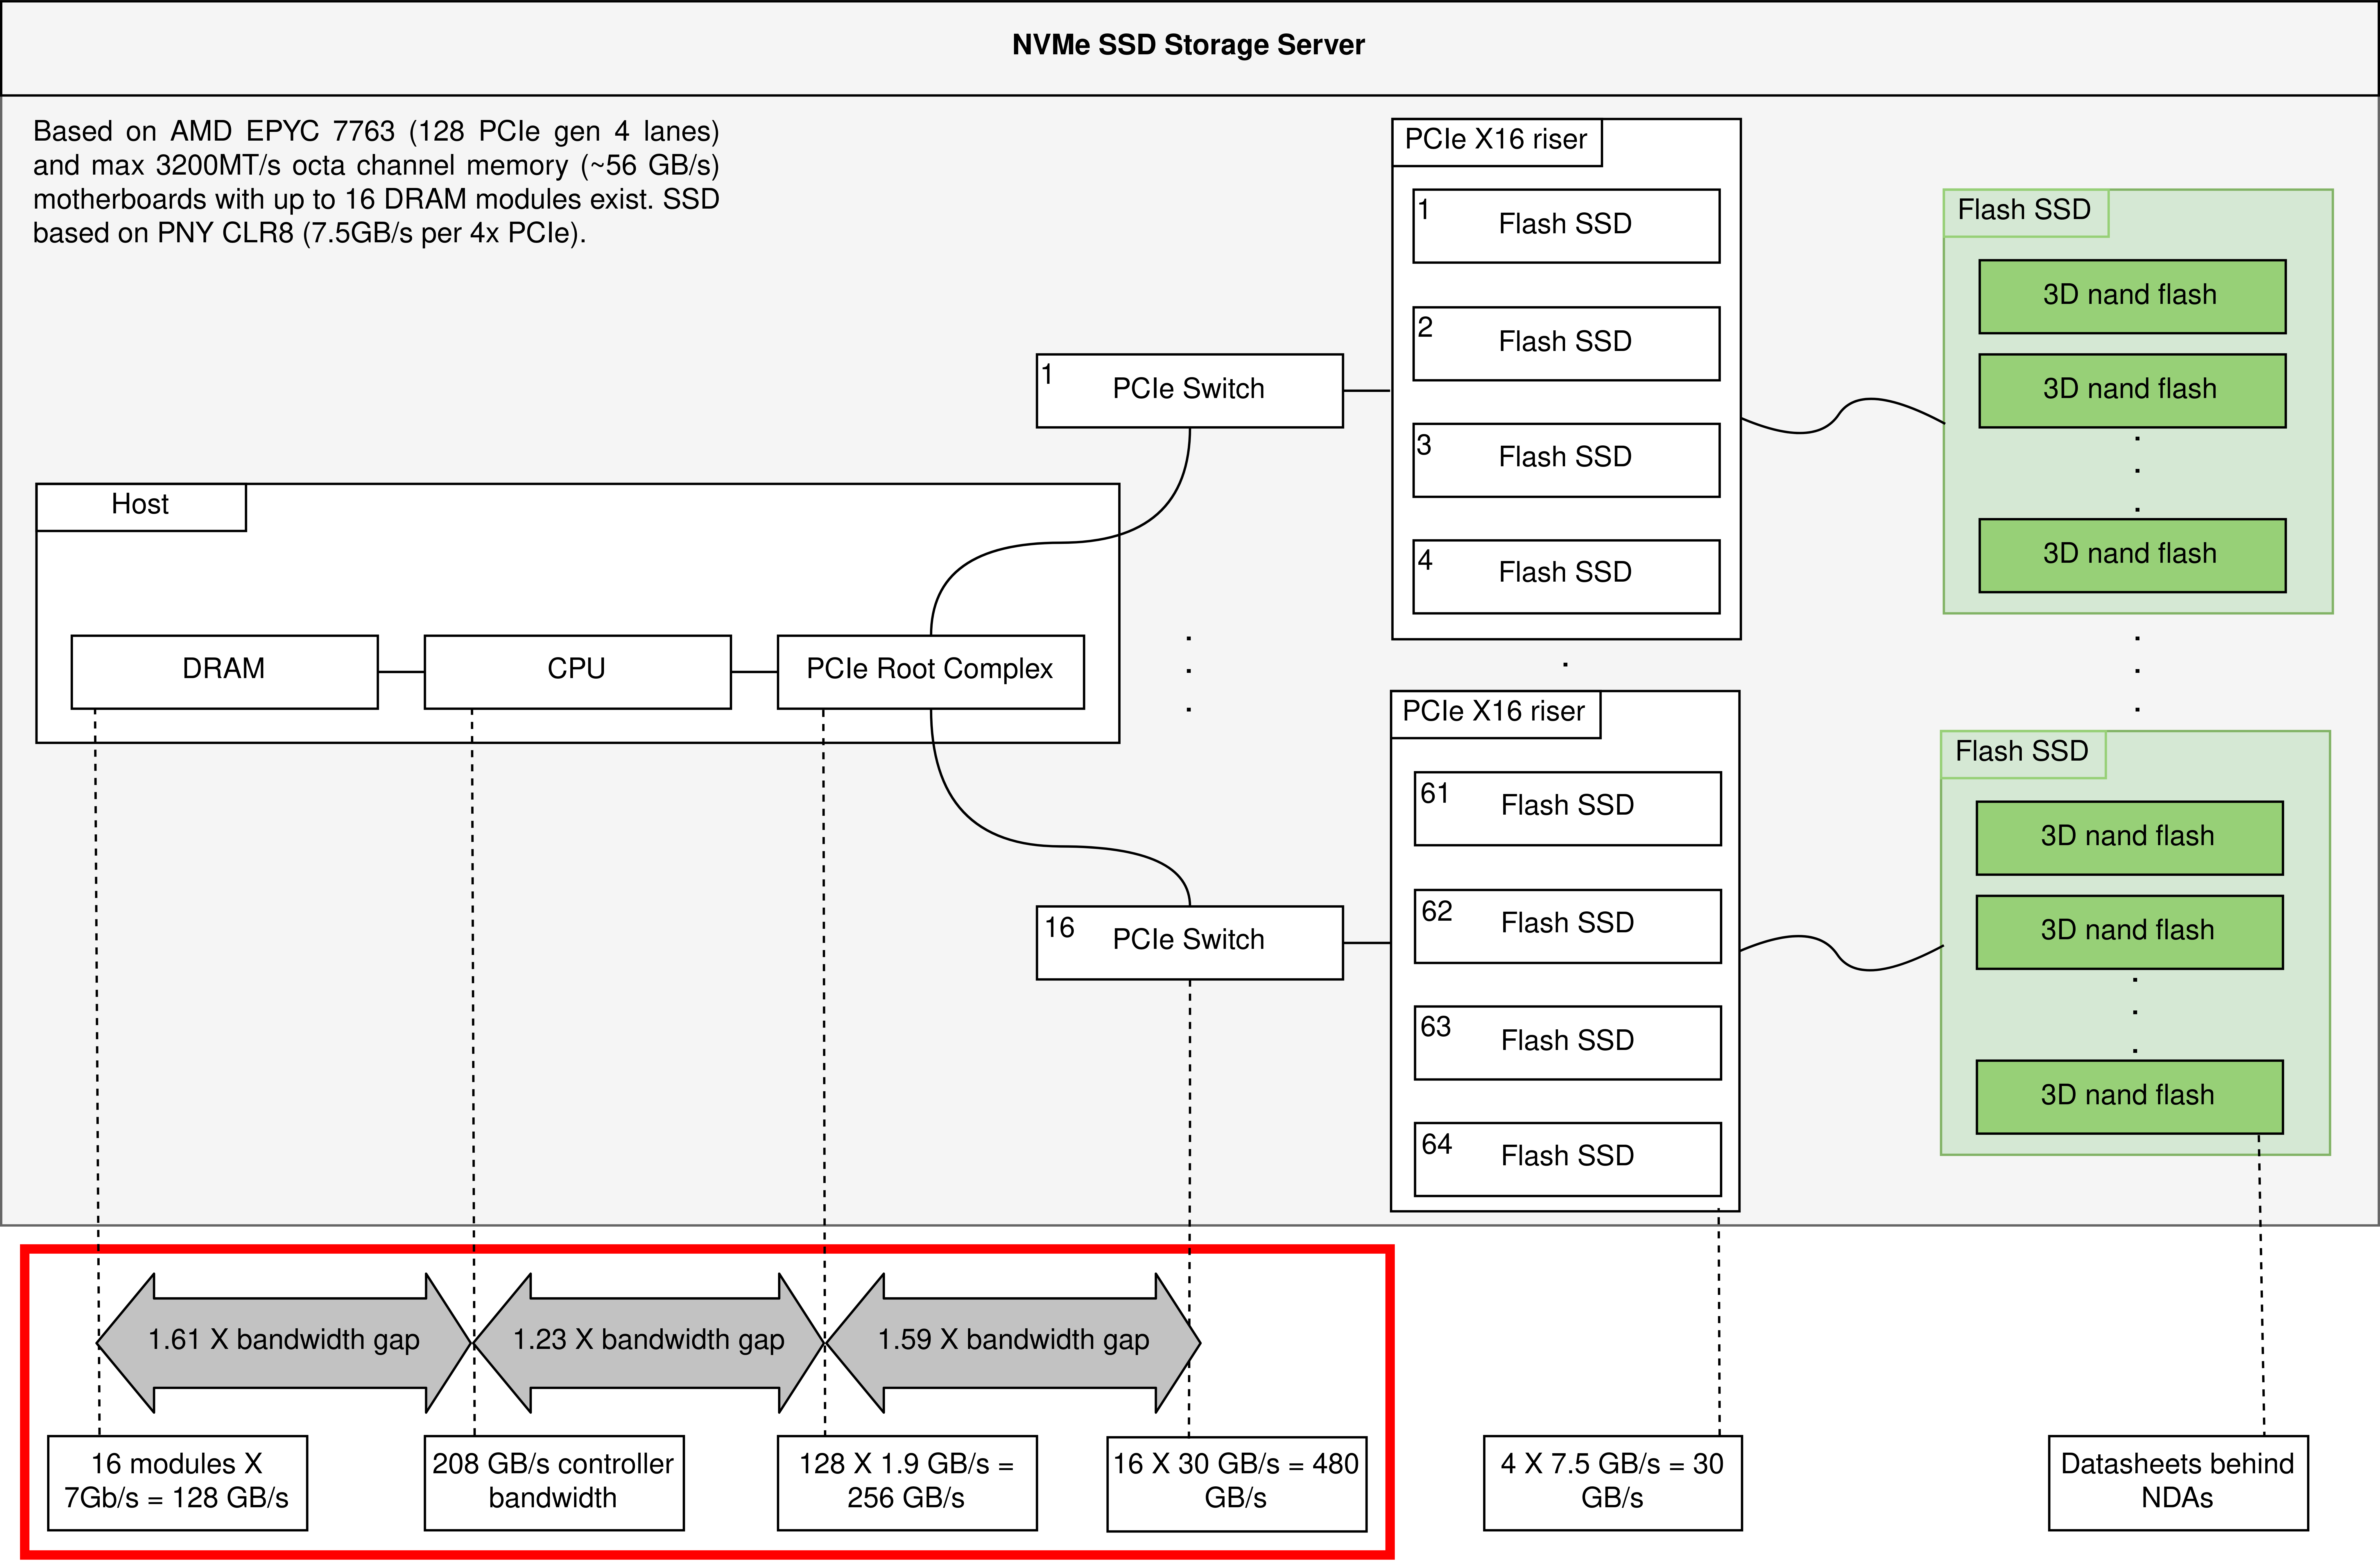
\includegraphics[width=0.87\textwidth]{resources/images/storage-bottleneck.png}
            \end{figure}
            \endgroup
        \end{column}
    \end{columns}
    \footnotetext[1]{\tiny https://www.kernel.org/doc/html/latest/driver-api/pci/p2pdma.html}
\end{frame}
\note{
    1m - 4.5
    \begin{itemize}
        \item Enterprise storage servers face large bandwidth gaps to meet
              economic densities.
        \item Actual bandwidth of flash chips on SSDs is often unknown.
        \item The PCIe root complex typically offers more bandwidth then the
              memory controller. Can be utilized by Peer-to-Peer DMA.
        \item p2p-dma across root complexes not supported by Linux due to
              optional support in specification.
    \end{itemize}
}

% page 3
\begin{frame}{What is Computational Storage}
    \begin{columns}
        \begin{column}{0.3\textwidth}
            \footnotesize
            \begin{itemize}
                \item Fit compute \& memory on storage device
                \item Specialized hardware (ASIC / FPGA)
                \item Improve energy efficiency
                \item Reduce data movement
                \item User submits programs to run on device (\textit{kernels})
            \end{itemize}
        \end{column}
        \begin{column}{0.7\textwidth}
            \begingroup
            \small
            \begin{figure}
                \centering
                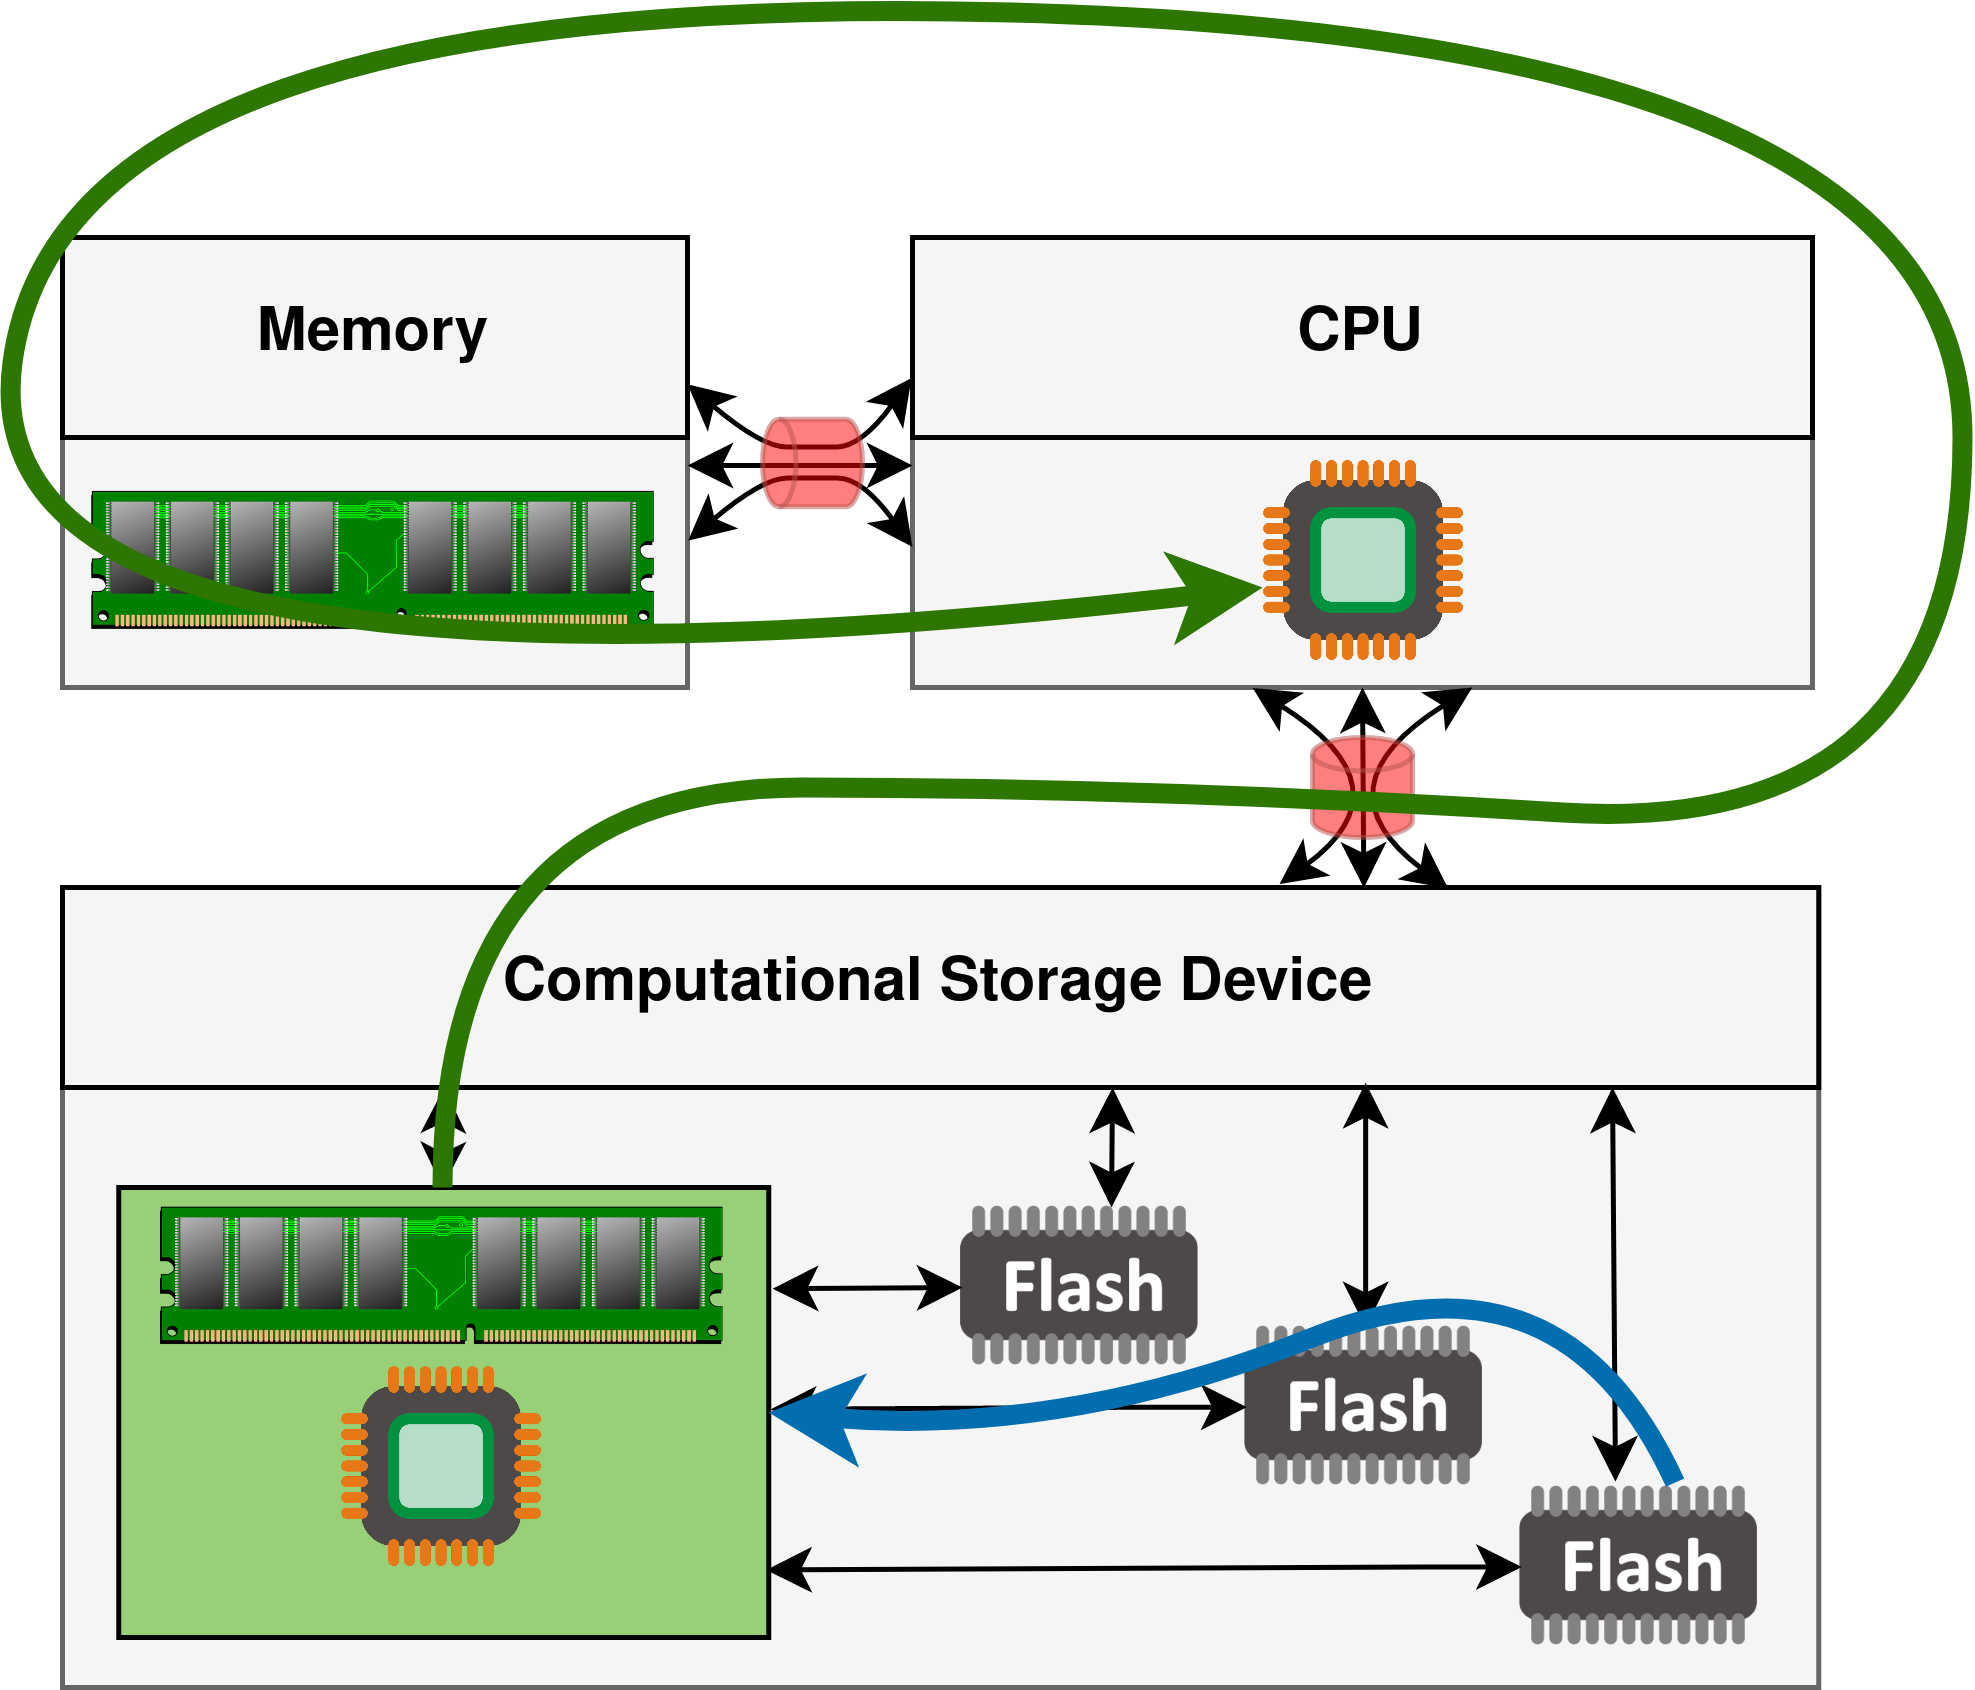
\includegraphics[width=0.7\textwidth]{resources/images/csd.png}
            \end{figure}
            \endgroup
        \end{column}
    \end{columns}
\end{frame}
\note{
    1m - 5.5
    \begin{itemize}
        \item Storage devices are fitted with their own computational elements
              and memory
        \item Often combination of regular processor and FPGA
        \item Host system sends user provided program to the device with metadata
        \item All data from storage moved internally to compute element
        \item Only result of computation moved over interconnect back to system
              memory.
        \item Results, in reduced energy consumption, occupied memory and
              peripheral bandwidth.
        \item Specialized lower performance cores often more energy efficient
              then high performance general performance.
    \end{itemize}
}

% % page 4
% % But such a heregoenous distributed system comes with many challenges and
% % complexities. Of which it be impossible to cover them all today. Instead we
% % focus on a prime example which is concurrent write modifcations to the same
% % file. How can we ensure that in multi-user tenant systems concurrent writes
% % partly on computational storage and partly executed by the host will not
% % override each others data. In the next slides some of the technologies used
% % to overcome this challenge are demonstrated.
% \begin{frame}{What is Computational Storage}
% 	\begingroup
% 	\small
% 	\begin{figure}
% 		\centering
% 		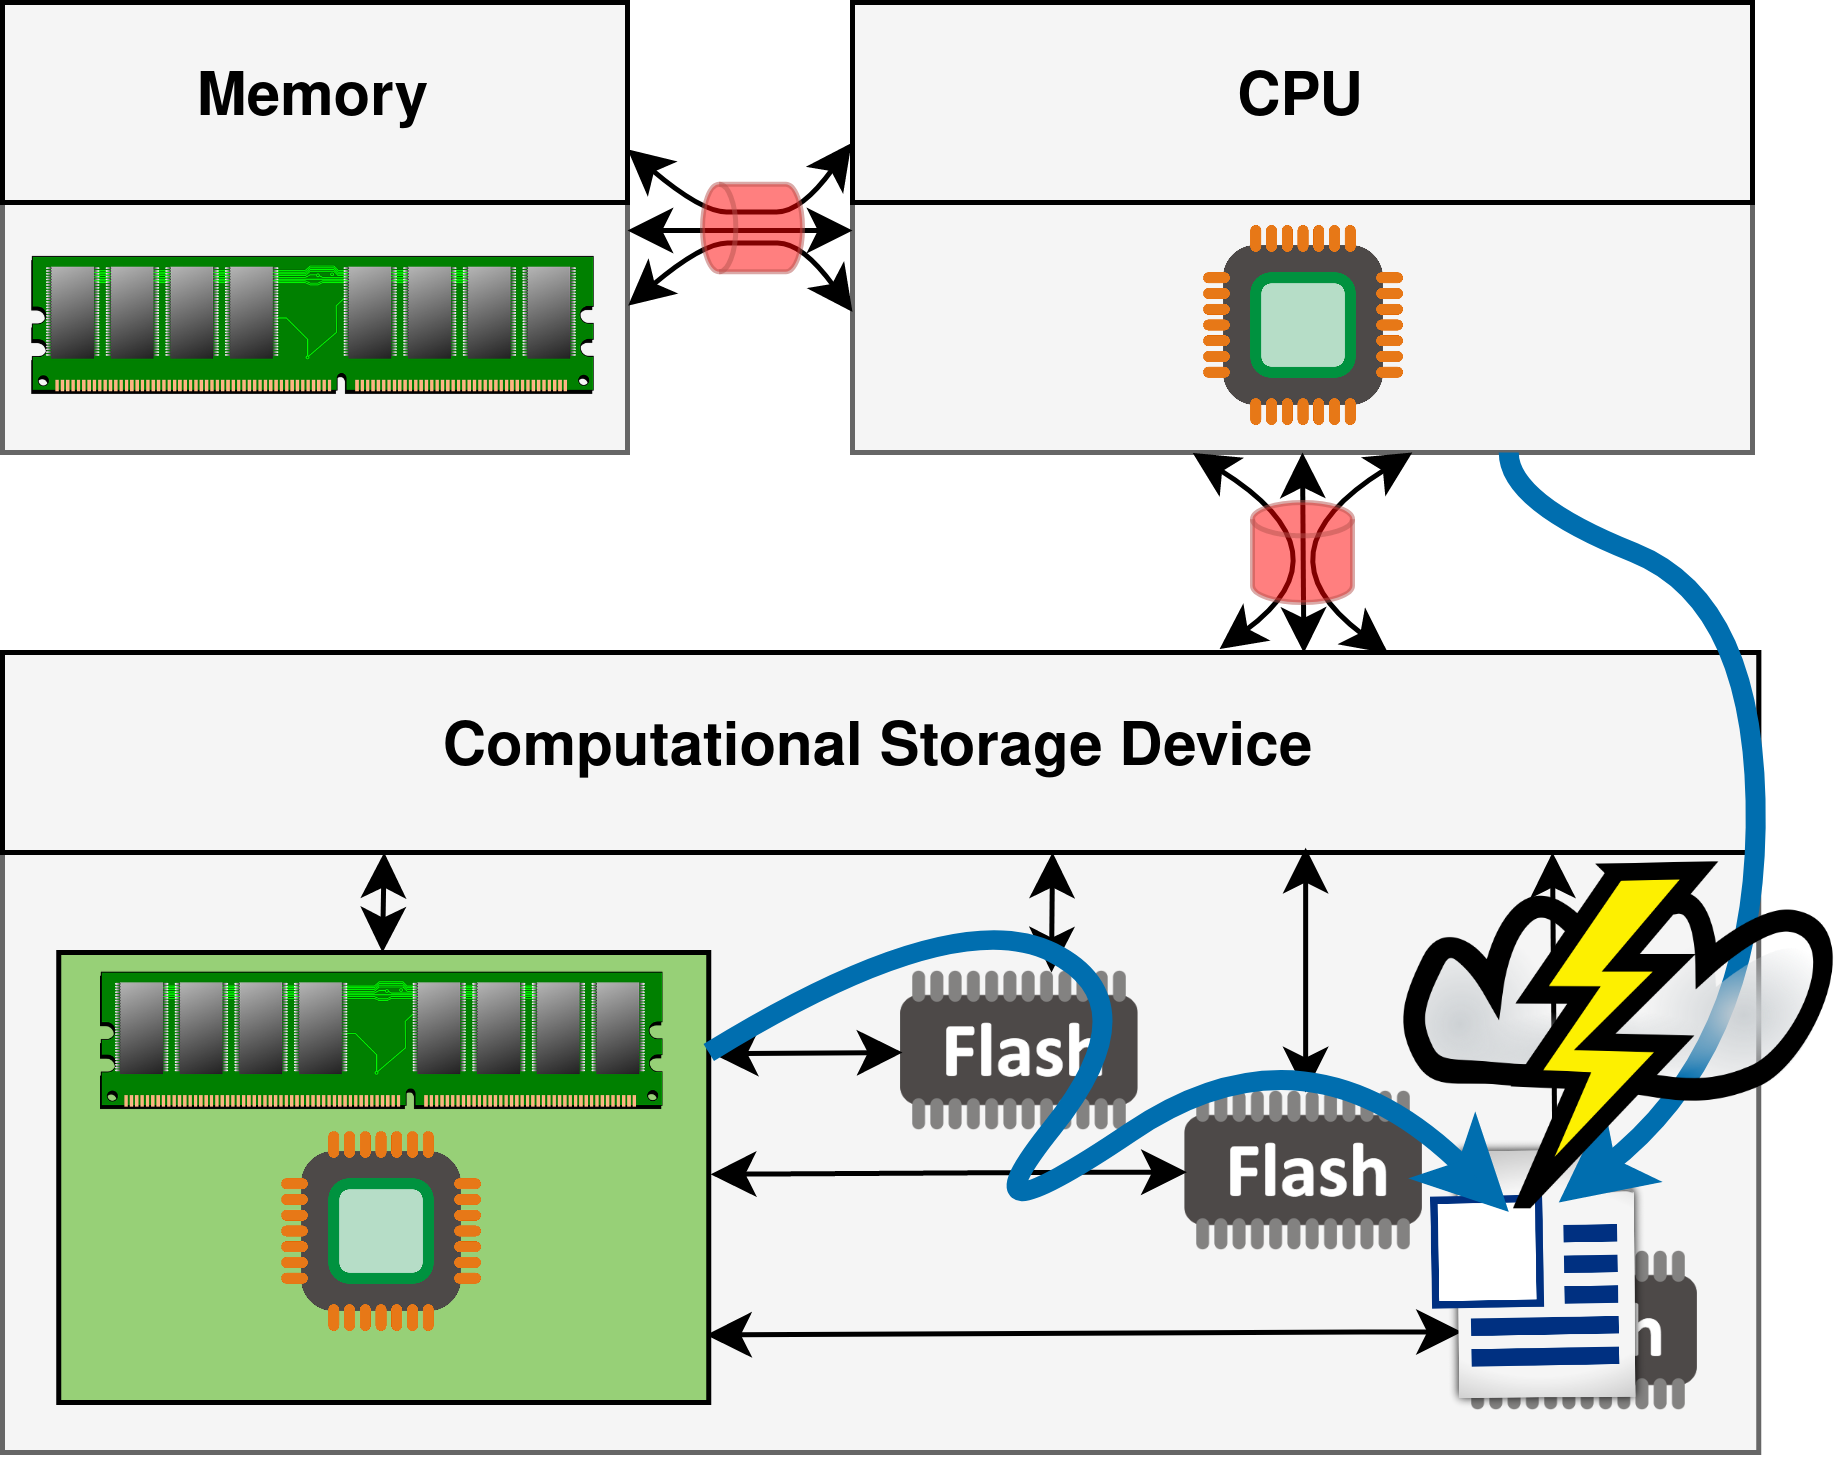
\includegraphics[width=0.7\textwidth]{resources/images/challenges.png}
% 	\end{figure}
% 	% \begin{itemize}
% 	% 	\item Von Neumann architecture
% 	% 	\item Memory bottlenecks
% 	% 	\item Energy efficiency
% 	% \end{itemize}
% 	\endgroup
% \end{frame}

\begin{frame}{State of Current Prototypes (September 2022)}
    \begin{columns}
        \begin{column}{0.5\textwidth}
            Shortlist:
            \footnotesize
            \begin{itemize}
                \item BlockNDP (2020) \footnotemark[2]
                \item Metal FS (2020) \footnotemark[3]
                \item INSIDER (July 2019) \footnotemark[4]
            \end{itemize}
        \end{column}
        \begin{column}{0.5\textwidth}
            Impediments:
            \footnotesize
            \begin{itemize}
                \item Lack of concurrent access
                \item Requires linking shared libraries
                \item Cumbersome interfaces
            \end{itemize}
        \end{column}
    \end{columns}
    \footnotetext[2]{\tiny https://doi.org/10.1145/3429357.3430519}
    \footnotetext[3]{\tiny https://doi.org/10.1145/3342195.3387557}
    \footnotetext[4]{\tiny https://www.usenix.org/conference/atc19/presentation/ruan}
\end{frame}
\note{
    1m - 6.5
    \begin{itemize}
        \item BlockNDP, designed for filesystem integration but never implemented
        \item Metal FS. overwrites default Linux pipe behavior
        \item INSIDER, requires linking a shared library
        \item None, support concurrent regular file and offloaded file access
        \item Interfaces often cumbersome, esoteric and unlike other filesystem
              interfaces.
    \end{itemize}
}

% \begin{frame}{Related Work}
%     \begin{columns}
%         \begin{column}{0.25\textwidth}
%             \footnotesize
%             \begin{itemize}
%                 \item Over a decade of research
%                 \item Many works, many different approaches
%                 \item Past survey for complete overview \footnotemark[5]
%             \end{itemize}
%         \end{column}
%         \begin{column}{0.75\textwidth}
%             \begingroup
%             \begin{figure}
%                 \centering
%                 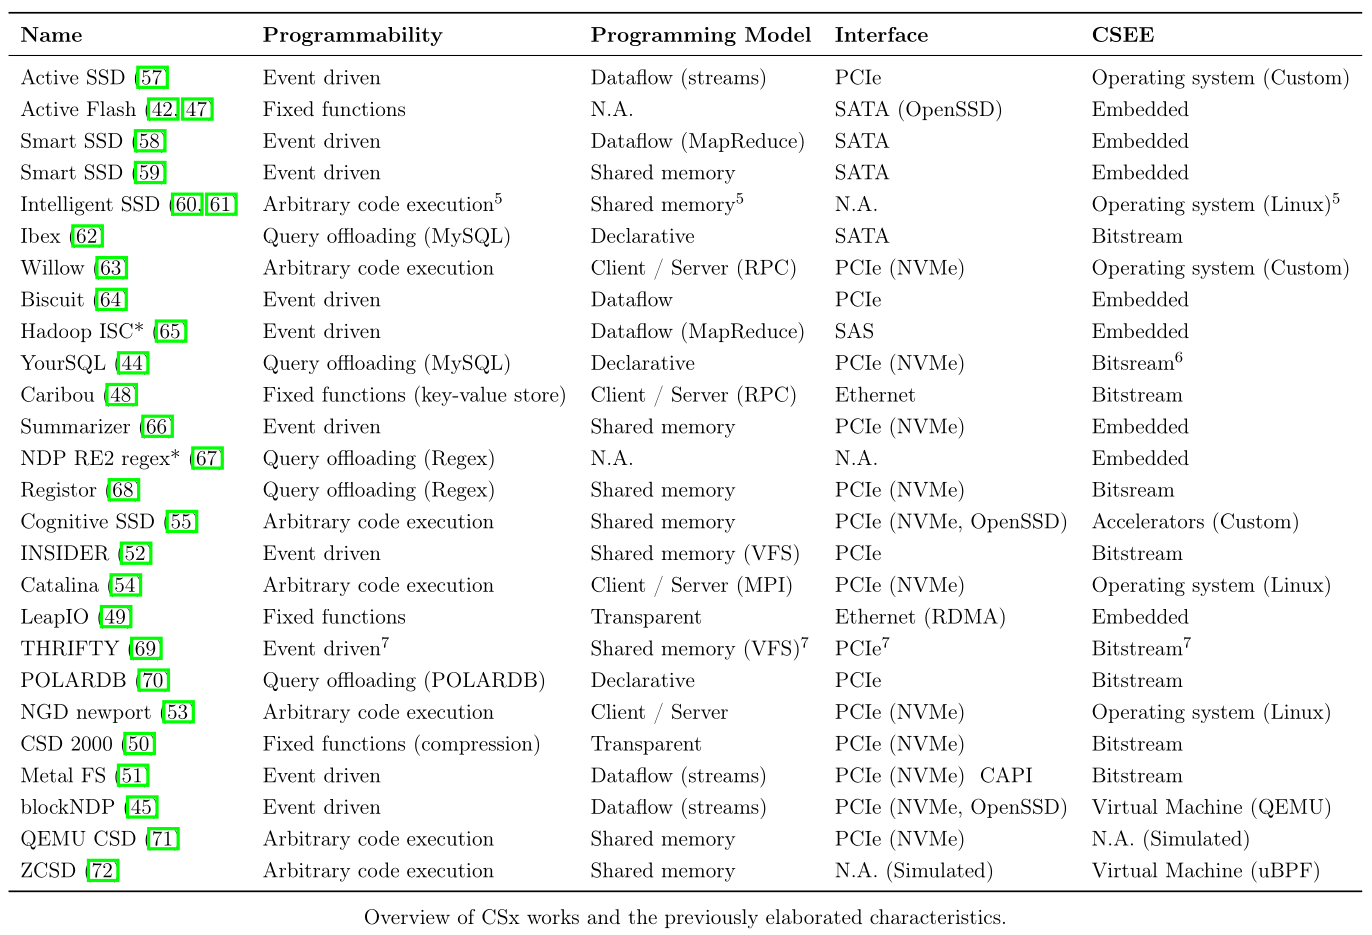
\includegraphics[width=0.8\textwidth]{resources/images/related-work.png}
%             \end{figure}
%             \endgroup
%         \end{column}
%     \end{columns}
%     \footnotetext[5]{\tiny https://arxiv.org/abs/2112.09691}
% \end{frame}
% \note{
%     30s - 7.0
%     \begin{itemize}
%         \item A little more of a complete overview
%         \item Ordered chronologically
%         \item Part of a bigger survey I did during my masters
%     \end{itemize}
% }

\begin{frame}{OpenCSD \& FluffleFS}
    \begin{columns}
        \begin{column}{0.45\textwidth}
            \footnotesize
            \begin{itemize}
                \item Entirely runs in user-space
                \item Using pre-existing system calls
                \item Concurrent access to same file
                \item Built using existing open-source libraries
                \item Use and experiment without any additional hardware
            \end{itemize}
        \end{column}
        \begin{column}{0.55\textwidth}
            \begin{figure}
                \centering
                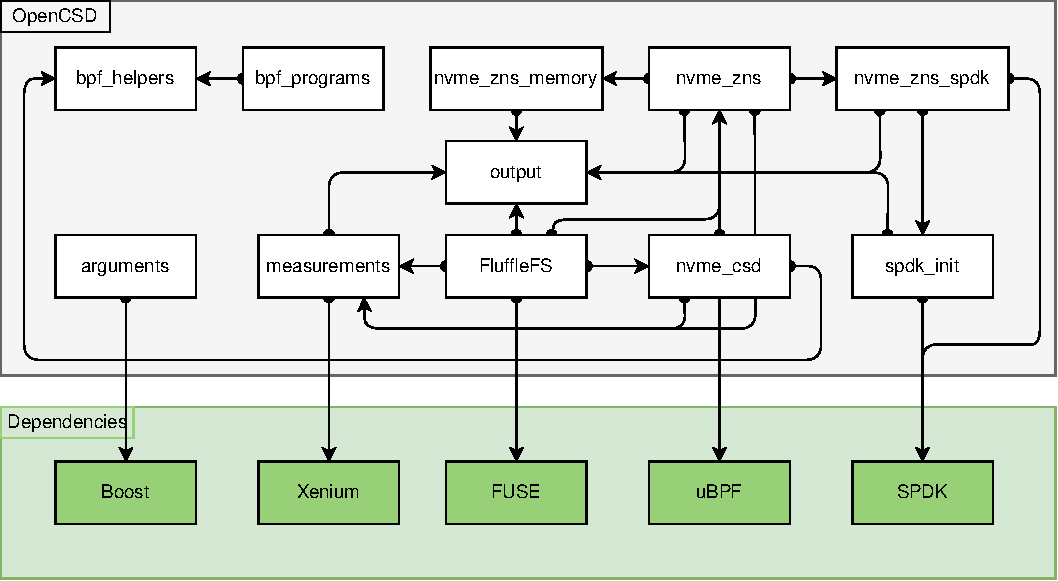
\includegraphics[width=1\textwidth]{resources/images/module-dependencies.pdf}
            \end{figure}
        \end{column}
    \end{columns}
\end{frame}
\note{
    1m - 8.0
    \begin{itemize}
        \item No kernel modules are required
        \item Use of system calls does not interfere with regular OS use
        \item First ever filesystem to support concurrent regular and offloaded
              access to the same file
        \item All features enabled by mixing the right pre-existing technologies
        \item Thanks to QEMU no additional hardware has to be purchased to try this
    \end{itemize}
}

% page 7
% To create such a filesystem our work relies on 5 fundamental design deicision
% and technologies. First is a software design using modules and interfaces this
% allows for rapid prototyping and loose coupling. Second is the use of a
% filesystem design from the 1990's a log-structured filesystem using append
% only writes. Third is the use of a new NVMe technology called Zoned Namespaces
% and fourth is the use of a filesystem feature supported by almost every
% filesystem even though not officially part of POSIX caled extended attributes.
\begin{frame}{Design}
	\begingroup
	\small

	\FourQuad%
		{\centering Modules \& Interfaces
		\begin{figure}
			\centering
			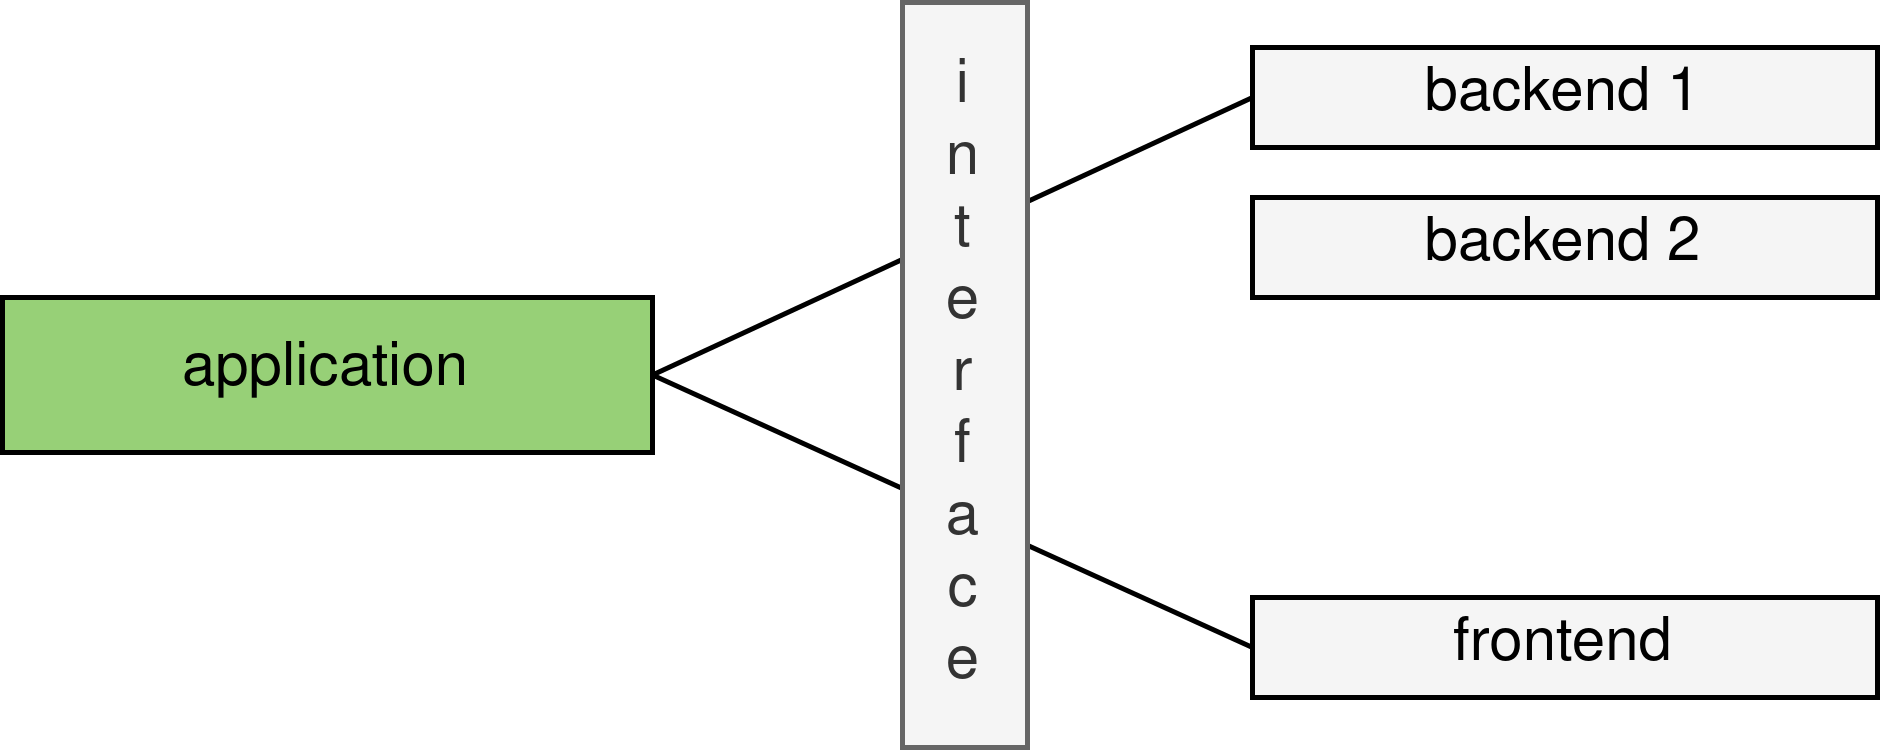
\includegraphics[width=0.85\textwidth]{resources/images/modules-interfaces.png}
		\end{figure}
		}
		{\centering Log-Structured Filesystem (LFS) \footnotemark[6]
		\begin{figure}
			\centering
			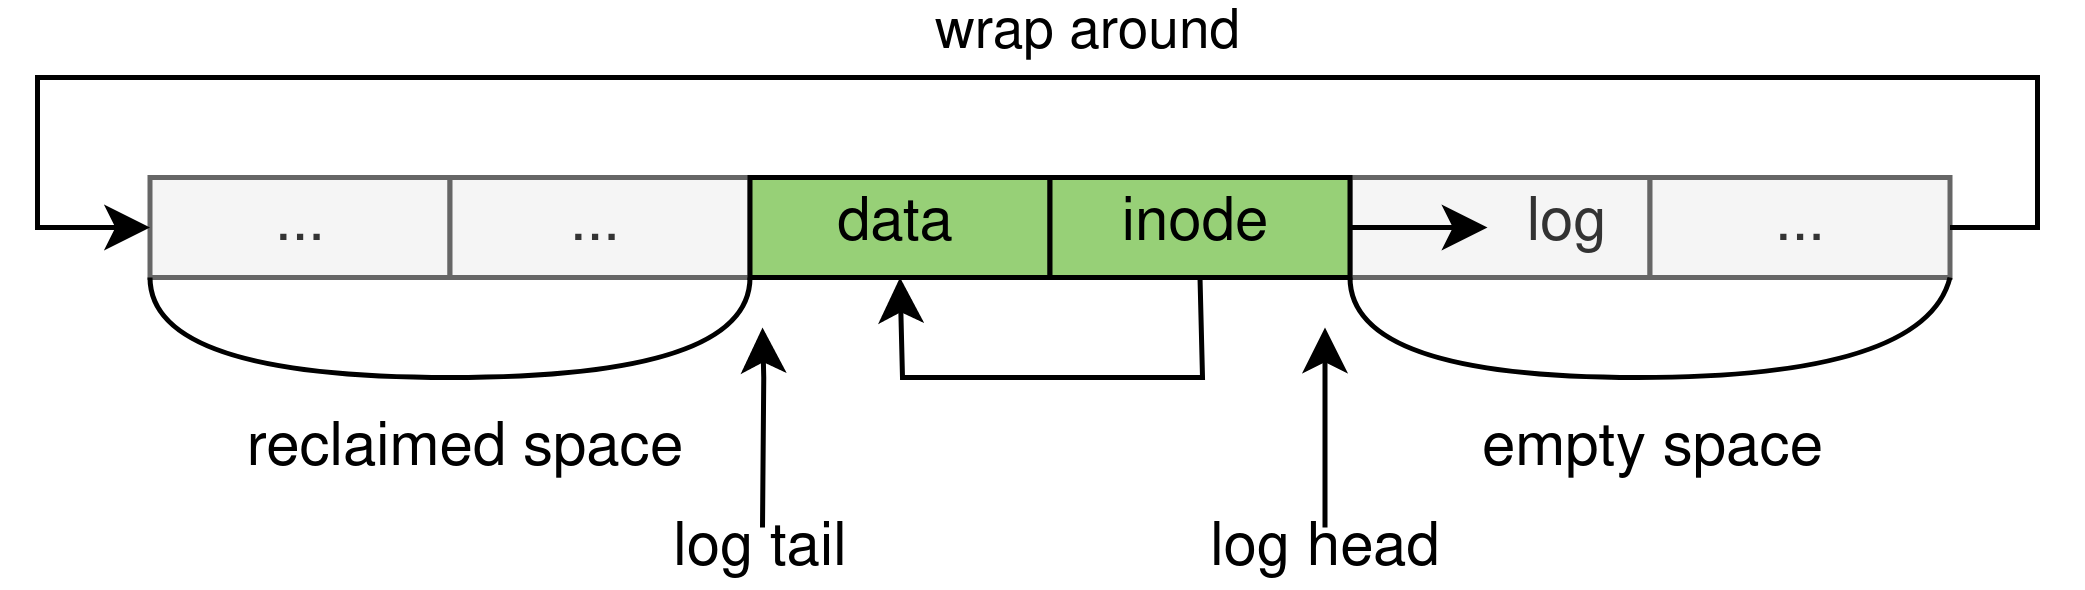
\includegraphics[width=0.9\textwidth]{resources/images/lfs-example.png}
		\end{figure}
		}
		{\centering Zoned Namespaces (ZNS)
		\begin{figure}
			\centering
			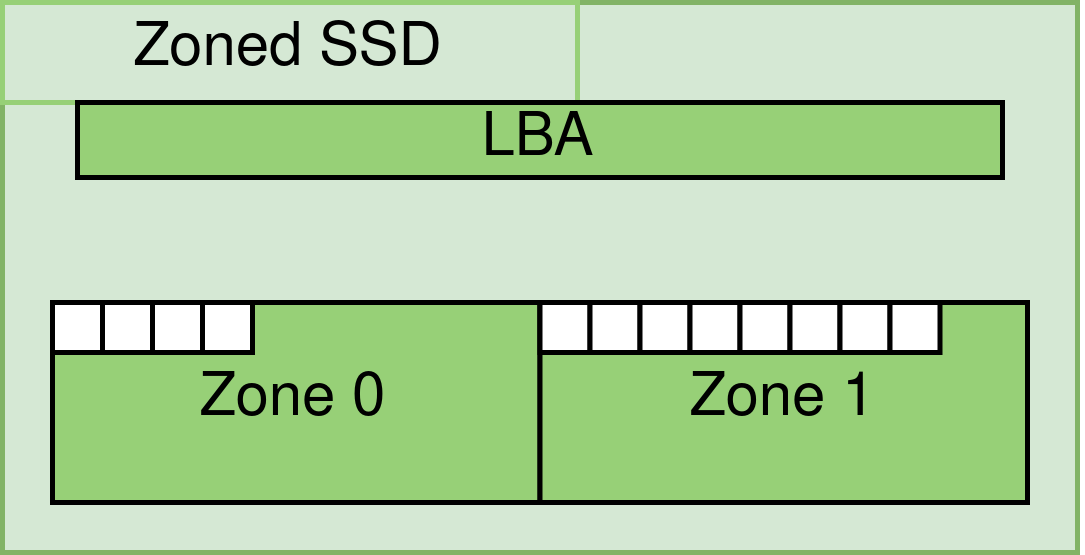
\includegraphics[width=0.55\textwidth]{resources/images/zns-simple.png}
		\end{figure}
		}
		{\centering Extended Attributes (xattr)
		\begin{figure}
			\centering
			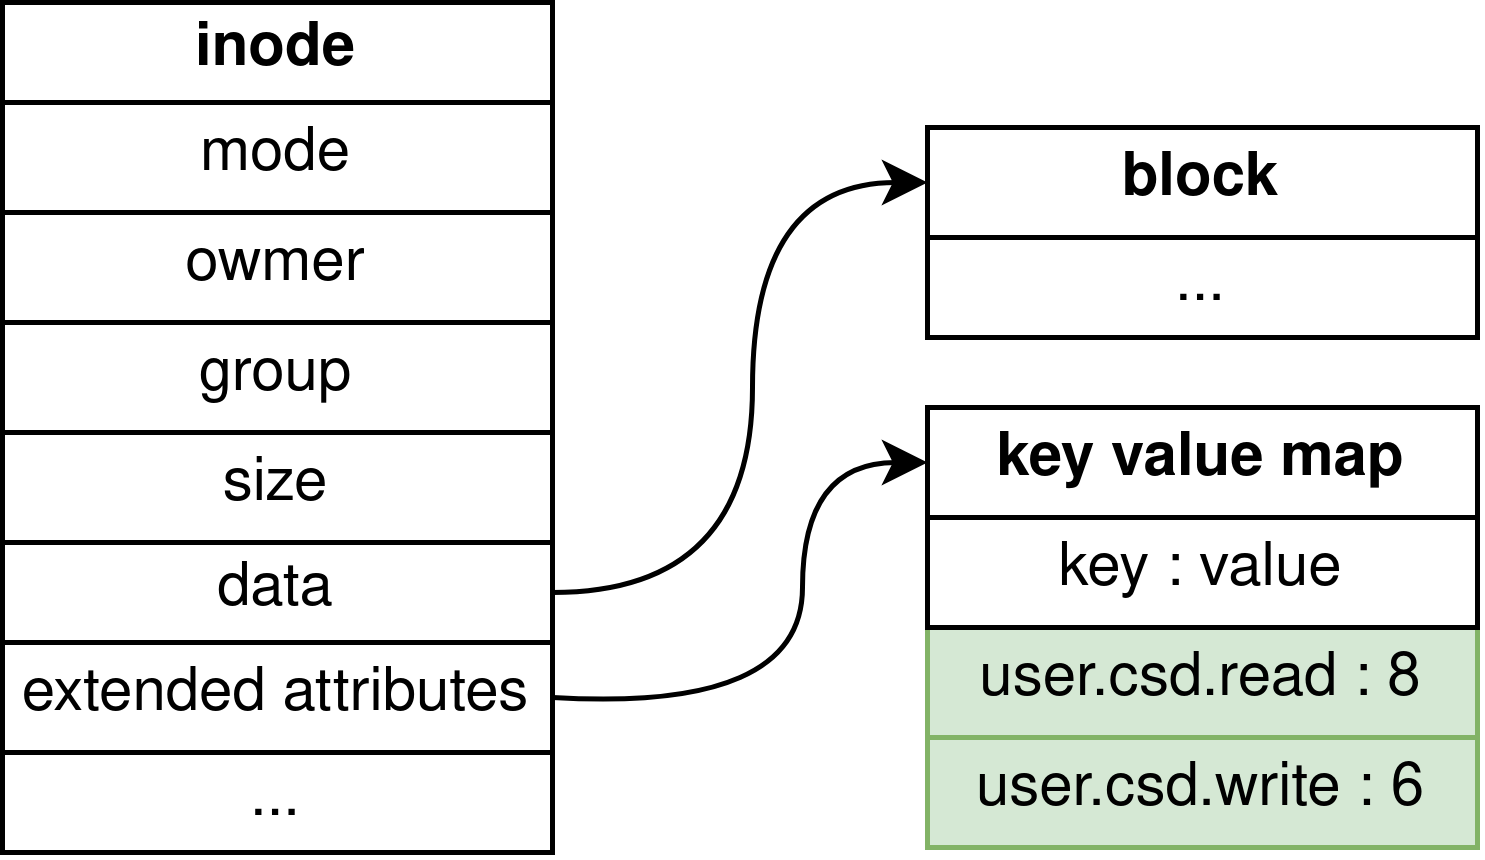
\includegraphics[width=0.65\textwidth]{resources/images/xattr-inode.png}
		\end{figure}
		}
		\footnotetext[6]{\tiny The design and implementation of a Log-structured File System}
	\endgroup
\end{frame}
\note{
    1m - 9.0
    \begin{itemize}
        \item Firstly, we separate the project into modules that can be combined
        \item Some modules, separate frontend and backends
        \item Allows to switch backend on the fly.
              Memory backed ZNS vs SPDK backend ZNS interface
        \item Use LFS, no in-place updates, write only append
        \item Will explain ZNS in more detail with some background on SSDs and
              the block interface.
        \item Extended attributes, system call allows to store arbitrary
              key-value pairs on individual files and folders. Present on
              basically any operating system (not POSIX).
    \end{itemize}
}

\begin{frame}{Design: Zoned NameSpaces (ZNS) 1/2}
    \begin{columns}
        \begin{column}{0.45\textwidth}
            \footnotesize
            Conventional SSDs
            \begin{itemize}
                \item The (traditional) block interface
                \item Linear writes
                \item Large erase units
                \item Flash Translation Layer (FTL)
                \item Logical vs Physical Block Address \\ (LBA / PBA)
            \end{itemize}
        \end{column}
        \begin{column}{0.55\textwidth}
            \begingroup
            \small
            \begin{figure}
                \centering
                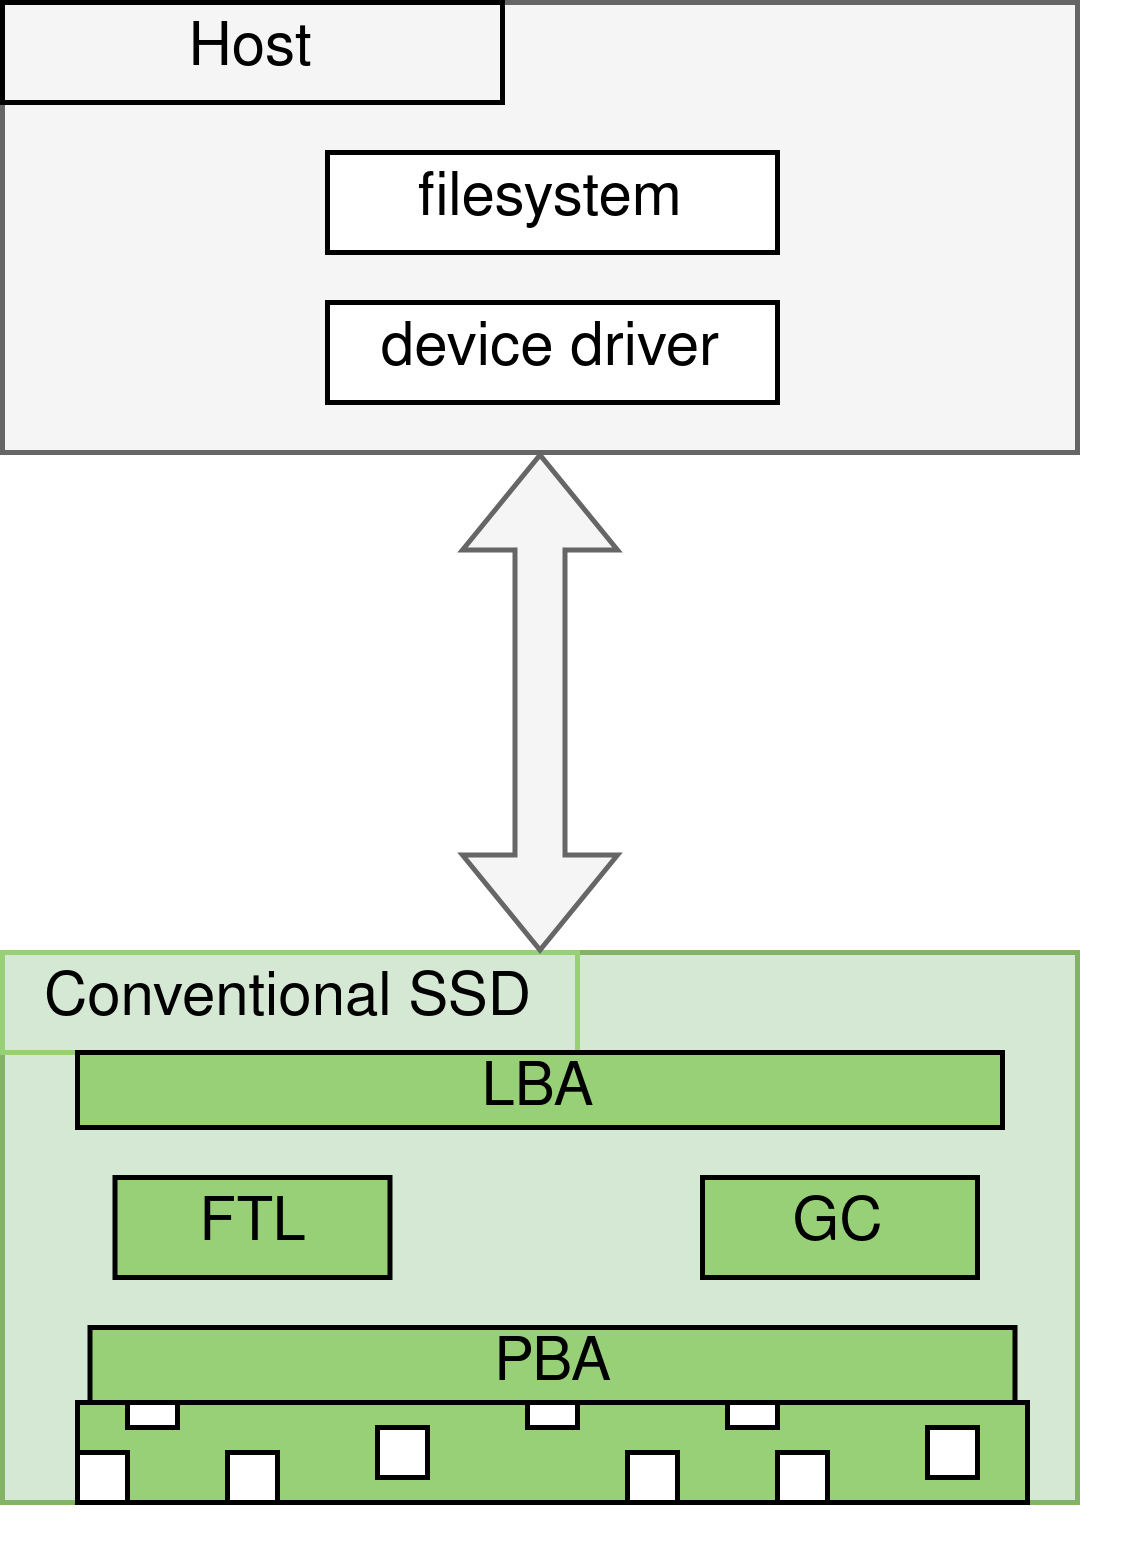
\includegraphics[width=0.5\textwidth]{resources/images/conventional.png}
            \end{figure}
            \endgroup
        \end{column}
    \end{columns}
\end{frame}
\note{
    1m - 11.0
    \begin{itemize}
        \item The block interface was created for hard-drives, spinning rust
        \item Any sector could be read and written in arbitrary fashion
        \item This same block interfaces was applied to SSDs
        \item However, SSD Nand Flash has much more restrictive properties
        \item In Nand flash every page / sector within a block needs to be
              linearly written
        \item Every block of sectors needs to be erased as a whole before
              it can be written again
        \item Since the block interface presents an arbitrary read / write
              interface the SSD needs to perform translations between the
              requested address and the actual address inside nand flash.
        \item This translation is known as the Flash Translation Layer (FTL)
              Reason most SSDs have relatively powerful microcontrollers.
    \end{itemize}
}

\begin{frame}{Design: Zoned NameSpaces (ZNS) \footnotemark[7] 2/2}
    \begin{columns}
        \begin{column}{0.45\textwidth}
            \footnotesize
            Zoned Namespaces SSDs
            \begin{itemize}
                \item Fit interface to nand flash behavior
                \item Devide erase units in zones
                \item Require each zone is linearly written
                \item Perfect match for LFS filesystems
                \item Host operating system manages FTL
            \end{itemize}
        \end{column}
        \begin{column}{0.55\textwidth}
            \begingroup
            \small
            \begin{figure}
                \centering
                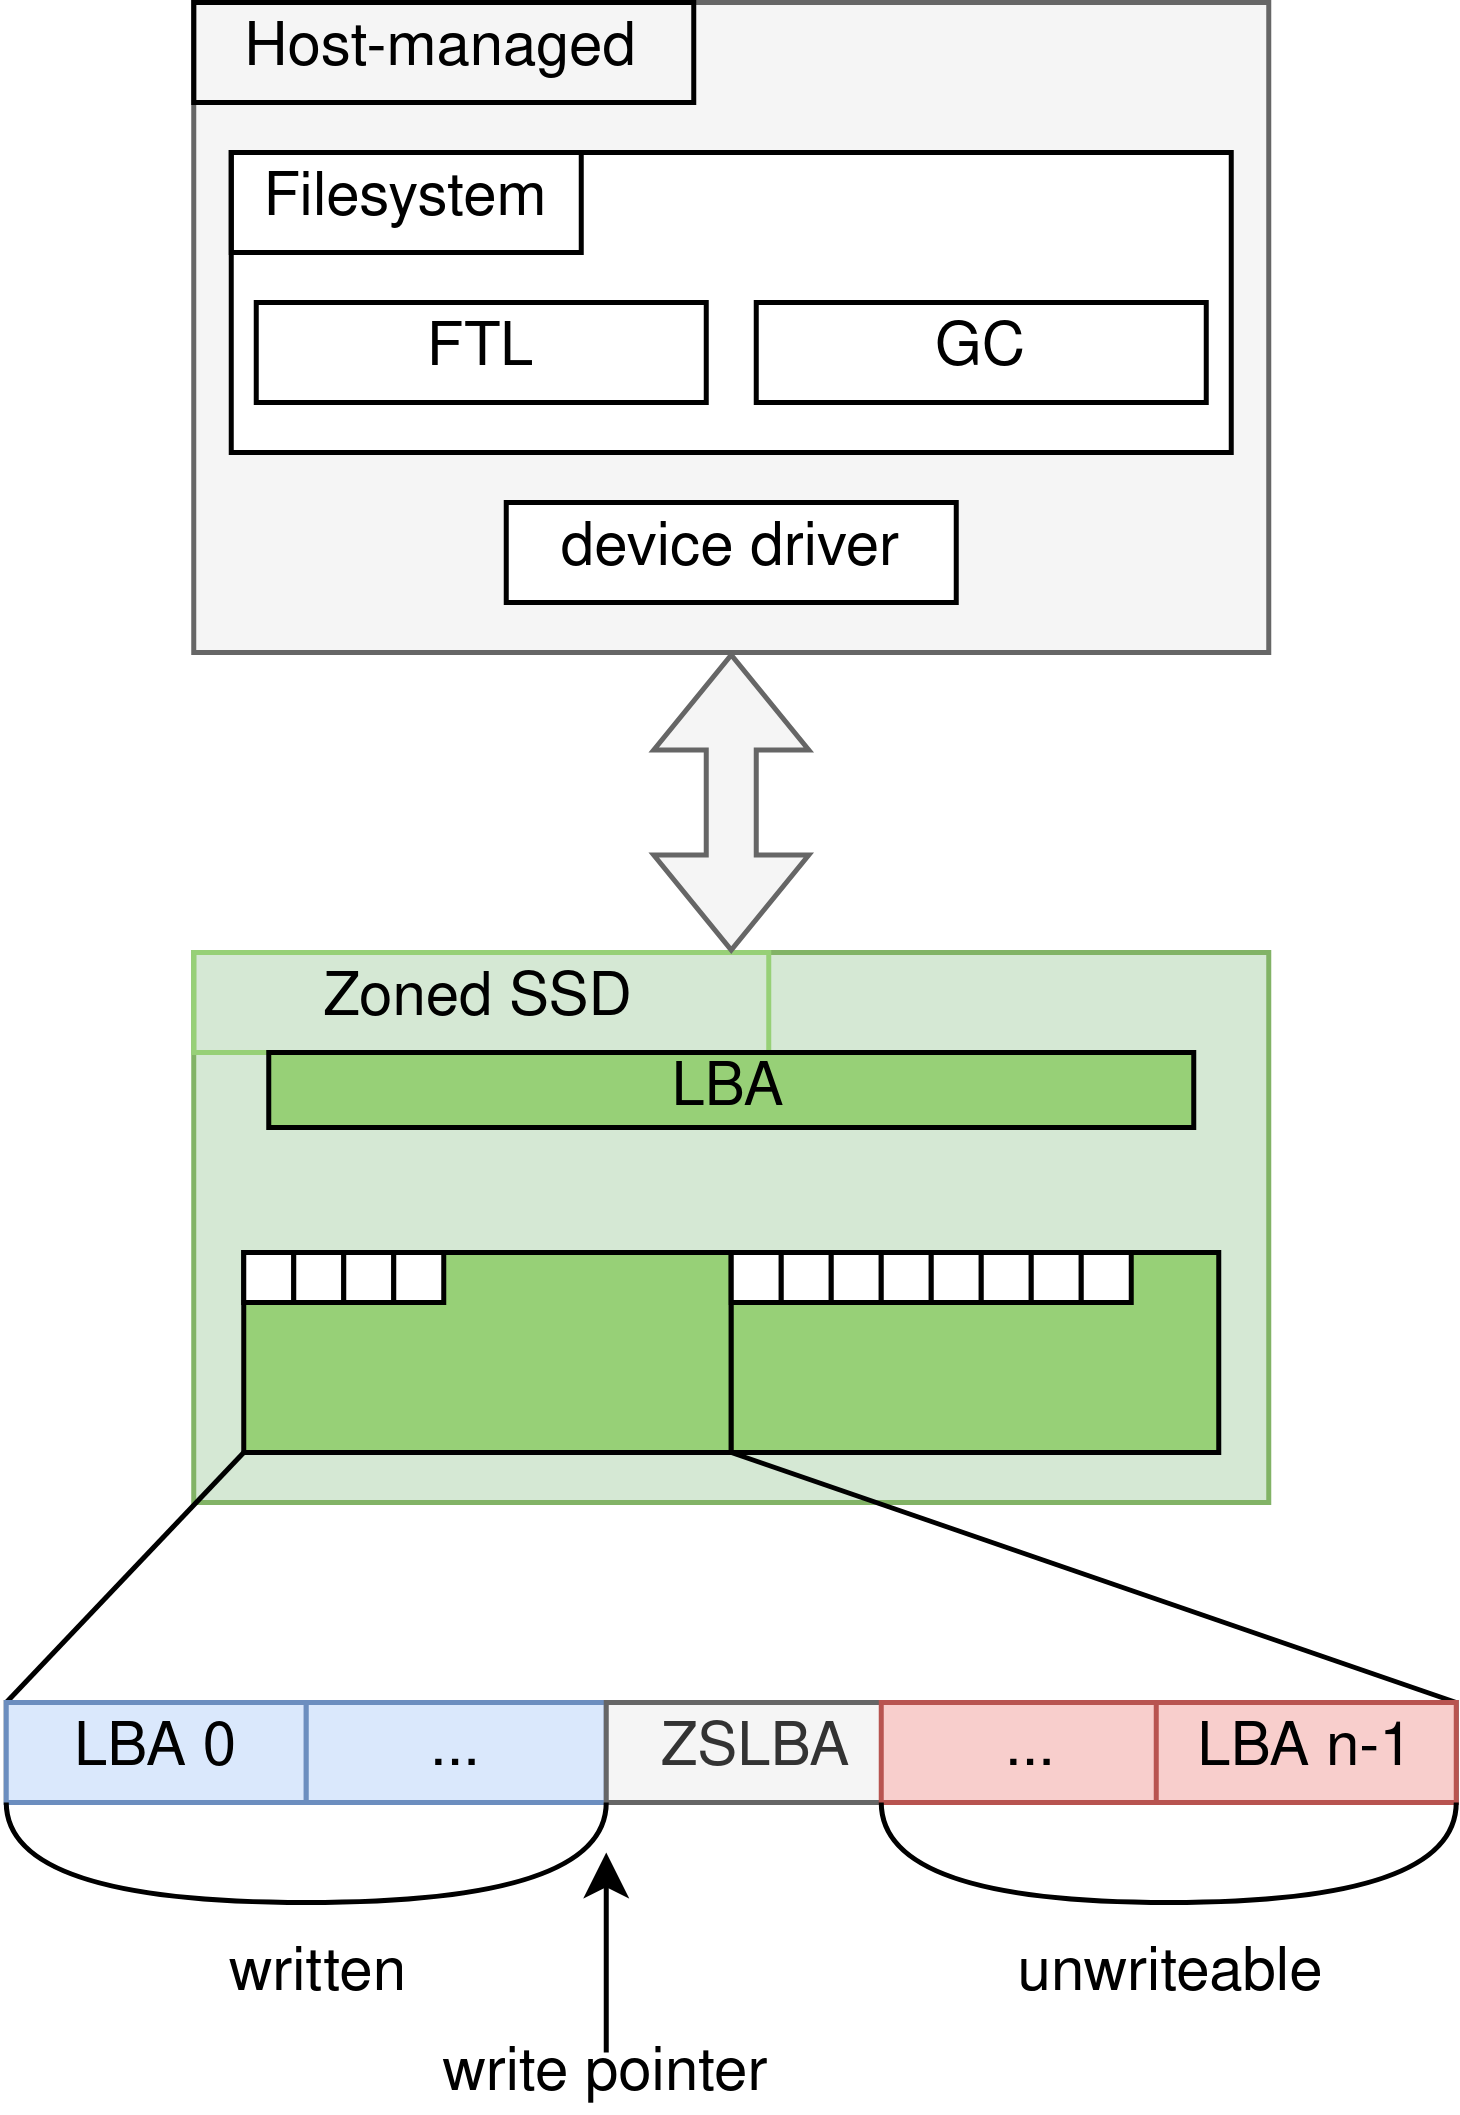
\includegraphics[width=0.5\textwidth]{resources/images/zns-lfs2.png}
            \end{figure}
            \endgroup
        \end{column}
    \end{columns}
    \footnotetext[7]{
        \tiny NVM Express Zoned Namespace Command Set Specification 1.1b -
        https://nvmexpress.org/developers/nvme-command-set-specifications/
    }
\end{frame}
\note{
    1m - 12.0
    \begin{itemize}
        \item Zoned Namespaces SSDs solves these issues with the block interface
        \item Allow the host to control data placement and decide when to perform
              erasure.
        \item No translation allows host filesystem to understand and reason
              about physical data location
        \item Absence of the FTL is critical for synchronising host
              filesystem with computational storage operations without expensive
              shared virtual memory.
    \end{itemize}
}

\begin{frame}{Design: ZNS + LFS}
    \begin{columns}
        \begin{column}{0.45\textwidth}
            \footnotesize
            Synchronizing host \& device filesystem
            \begin{itemize}
                \item Ensure file immutable for kernels
                \item No host communication during kernel execution
                \item Unblock regular access
                \item Check \& understand kernel behavior
            \end{itemize}
            \textit{Snapshot consistency model}
        \end{column}
        \begin{column}{0.55\textwidth}
            \begingroup
            \small
            \begin{figure}
                \centering
                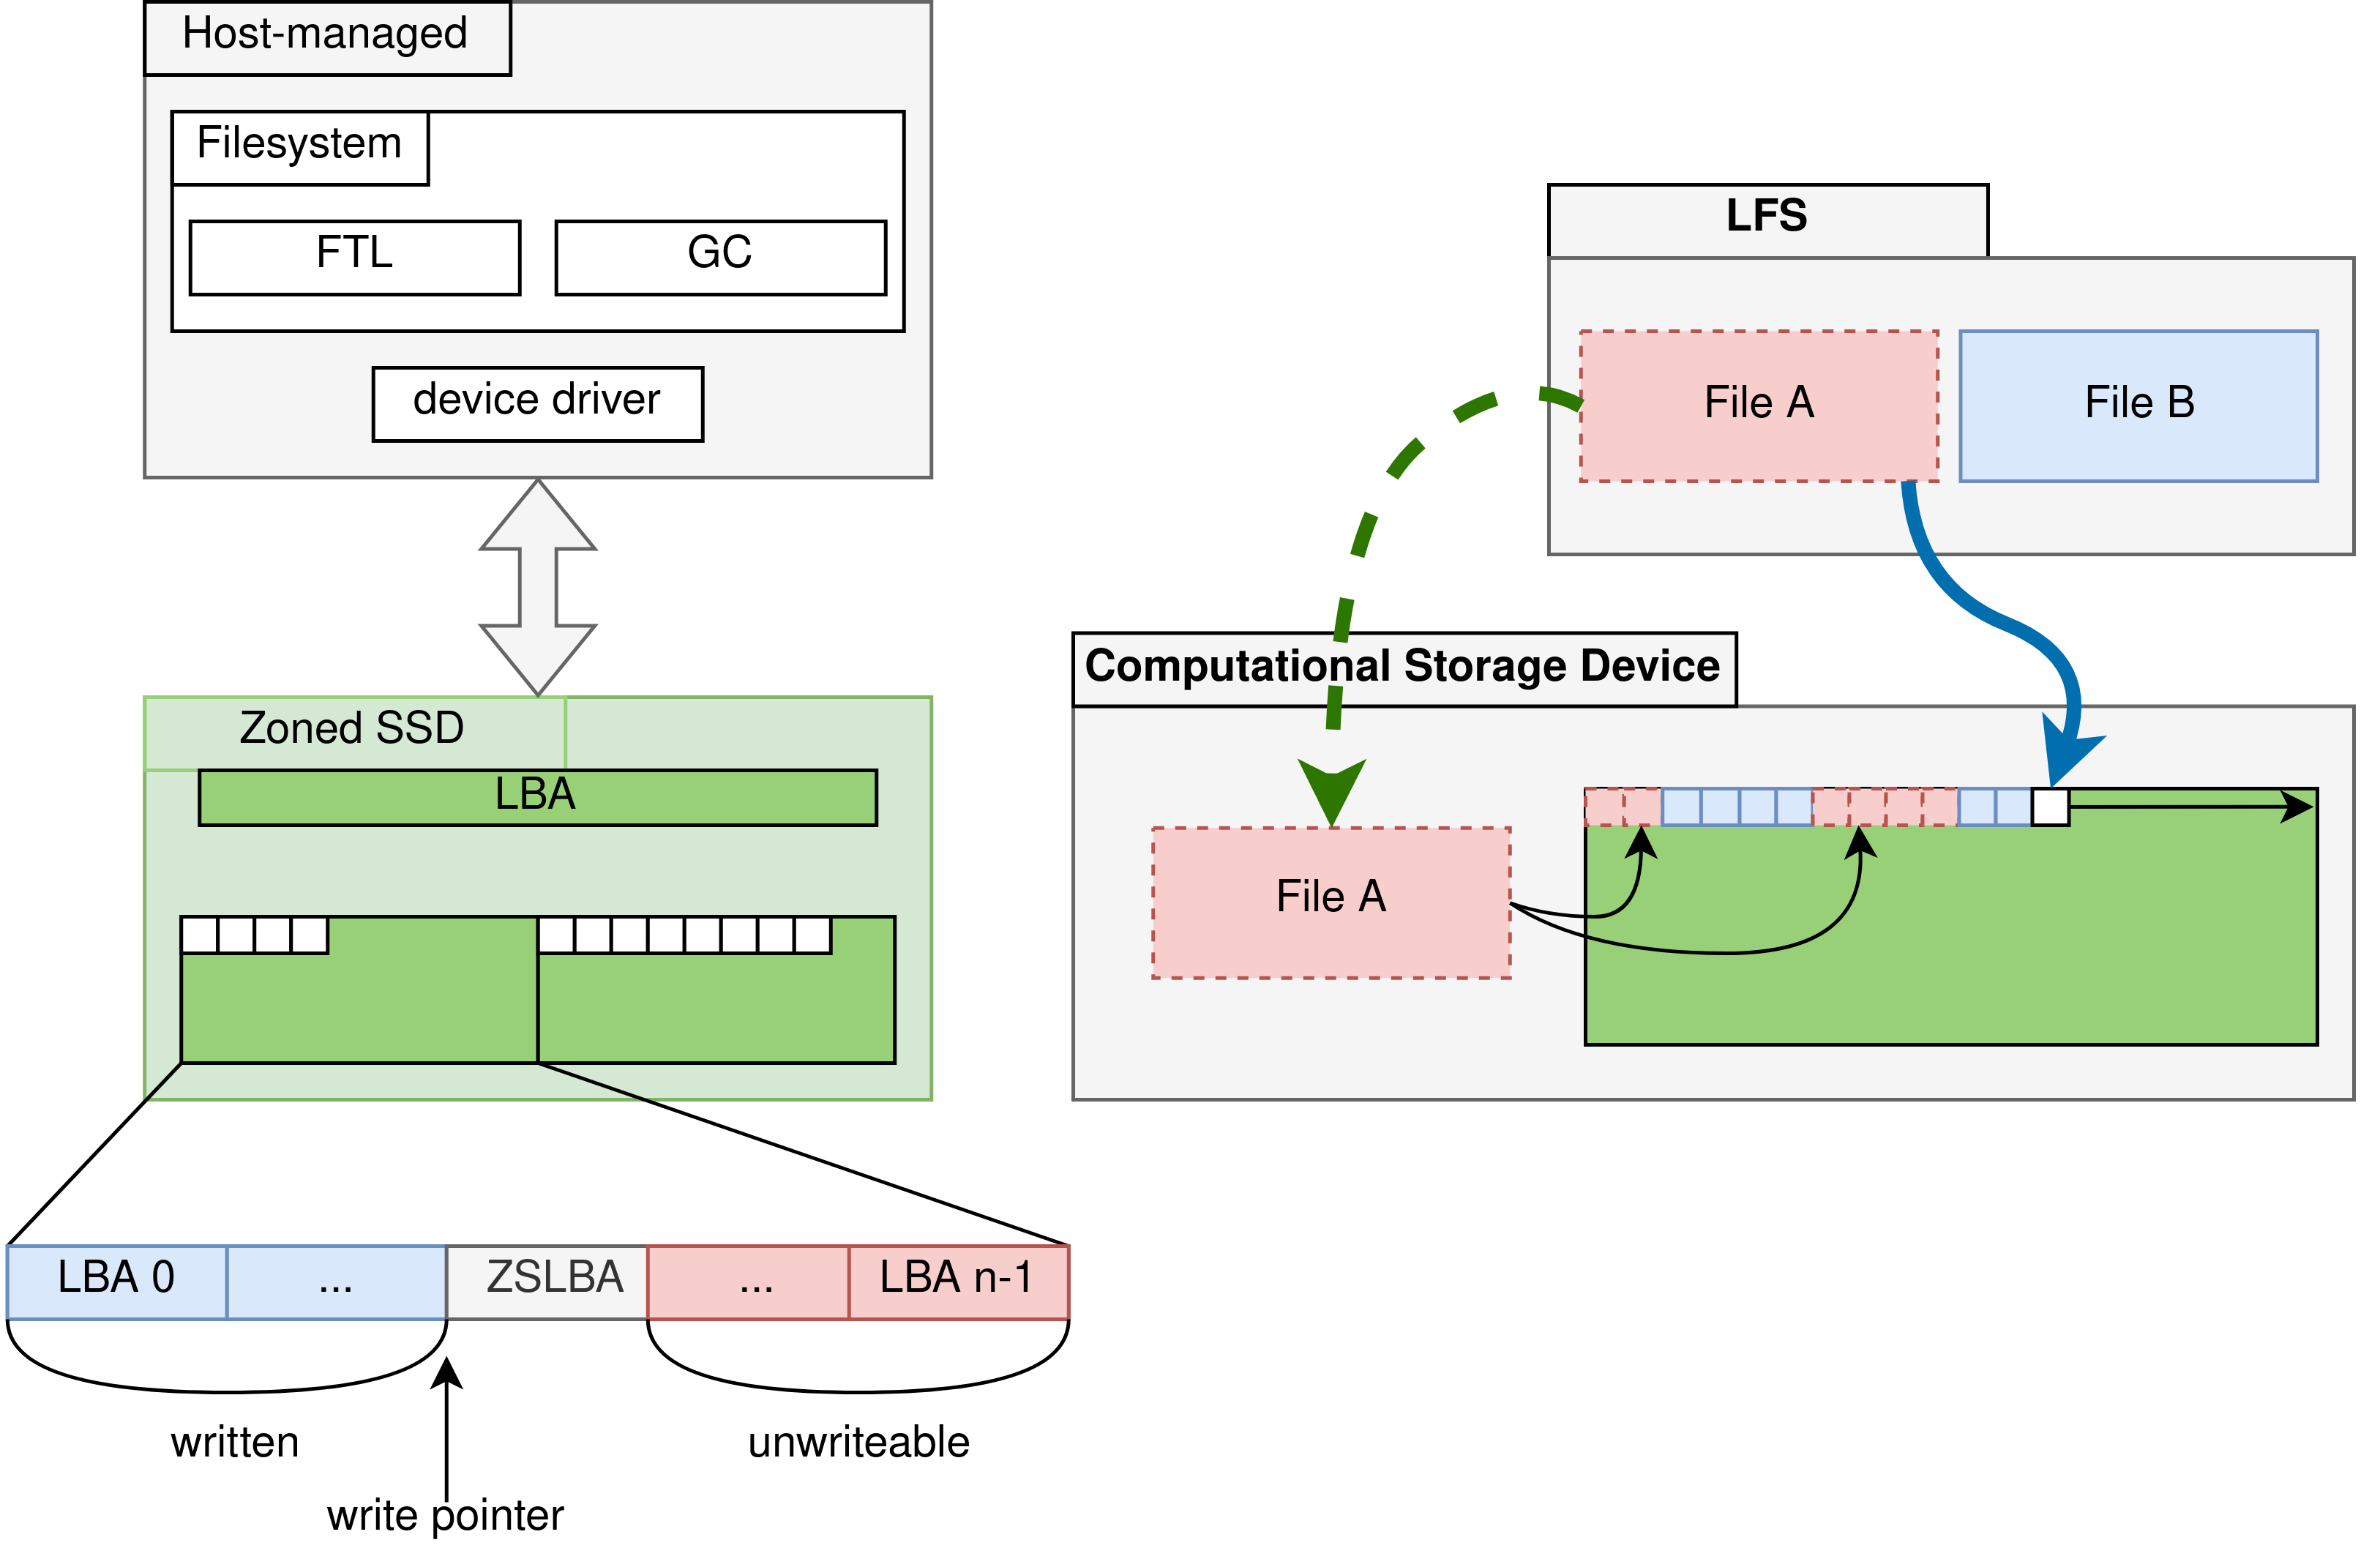
\includegraphics[width=1\textwidth]{resources/images/zns-lfs3.png}
            \end{figure}
            \endgroup
        \end{column}
    \end{columns}
\end{frame}
\note{
    1.5m - 13.5
    \begin{itemize}
        \item Cache-coherent interconnects exist / shared virtual memory exists,
              not the point won't be performant due to roundtrip time.
        \item In-memory snapshots solve all these issues.
        \item Send metadata of file, block locations etc, permissions for kernel
              along with the kernel and I/O request.
    \end{itemize}
}

\begin{frame}{Design: Architecture Independent Kernels}
    \begin{columns}
        \begin{column}{0.45\textwidth}
            \footnotesize
            \begin{itemize}
                \item Define system calls in ABI header
                \item Leave implementation to VM (vendor)
                \item Compile once use everywhere
                \item eBPF ISA trivial to implement in VM
                \item Pre-existing FOSS eBPF VMs (uBPF)
            \end{itemize}
        \end{column}
        \begin{column}{0.55\textwidth}
            \begingroup
            \begin{figure}
                \centering
                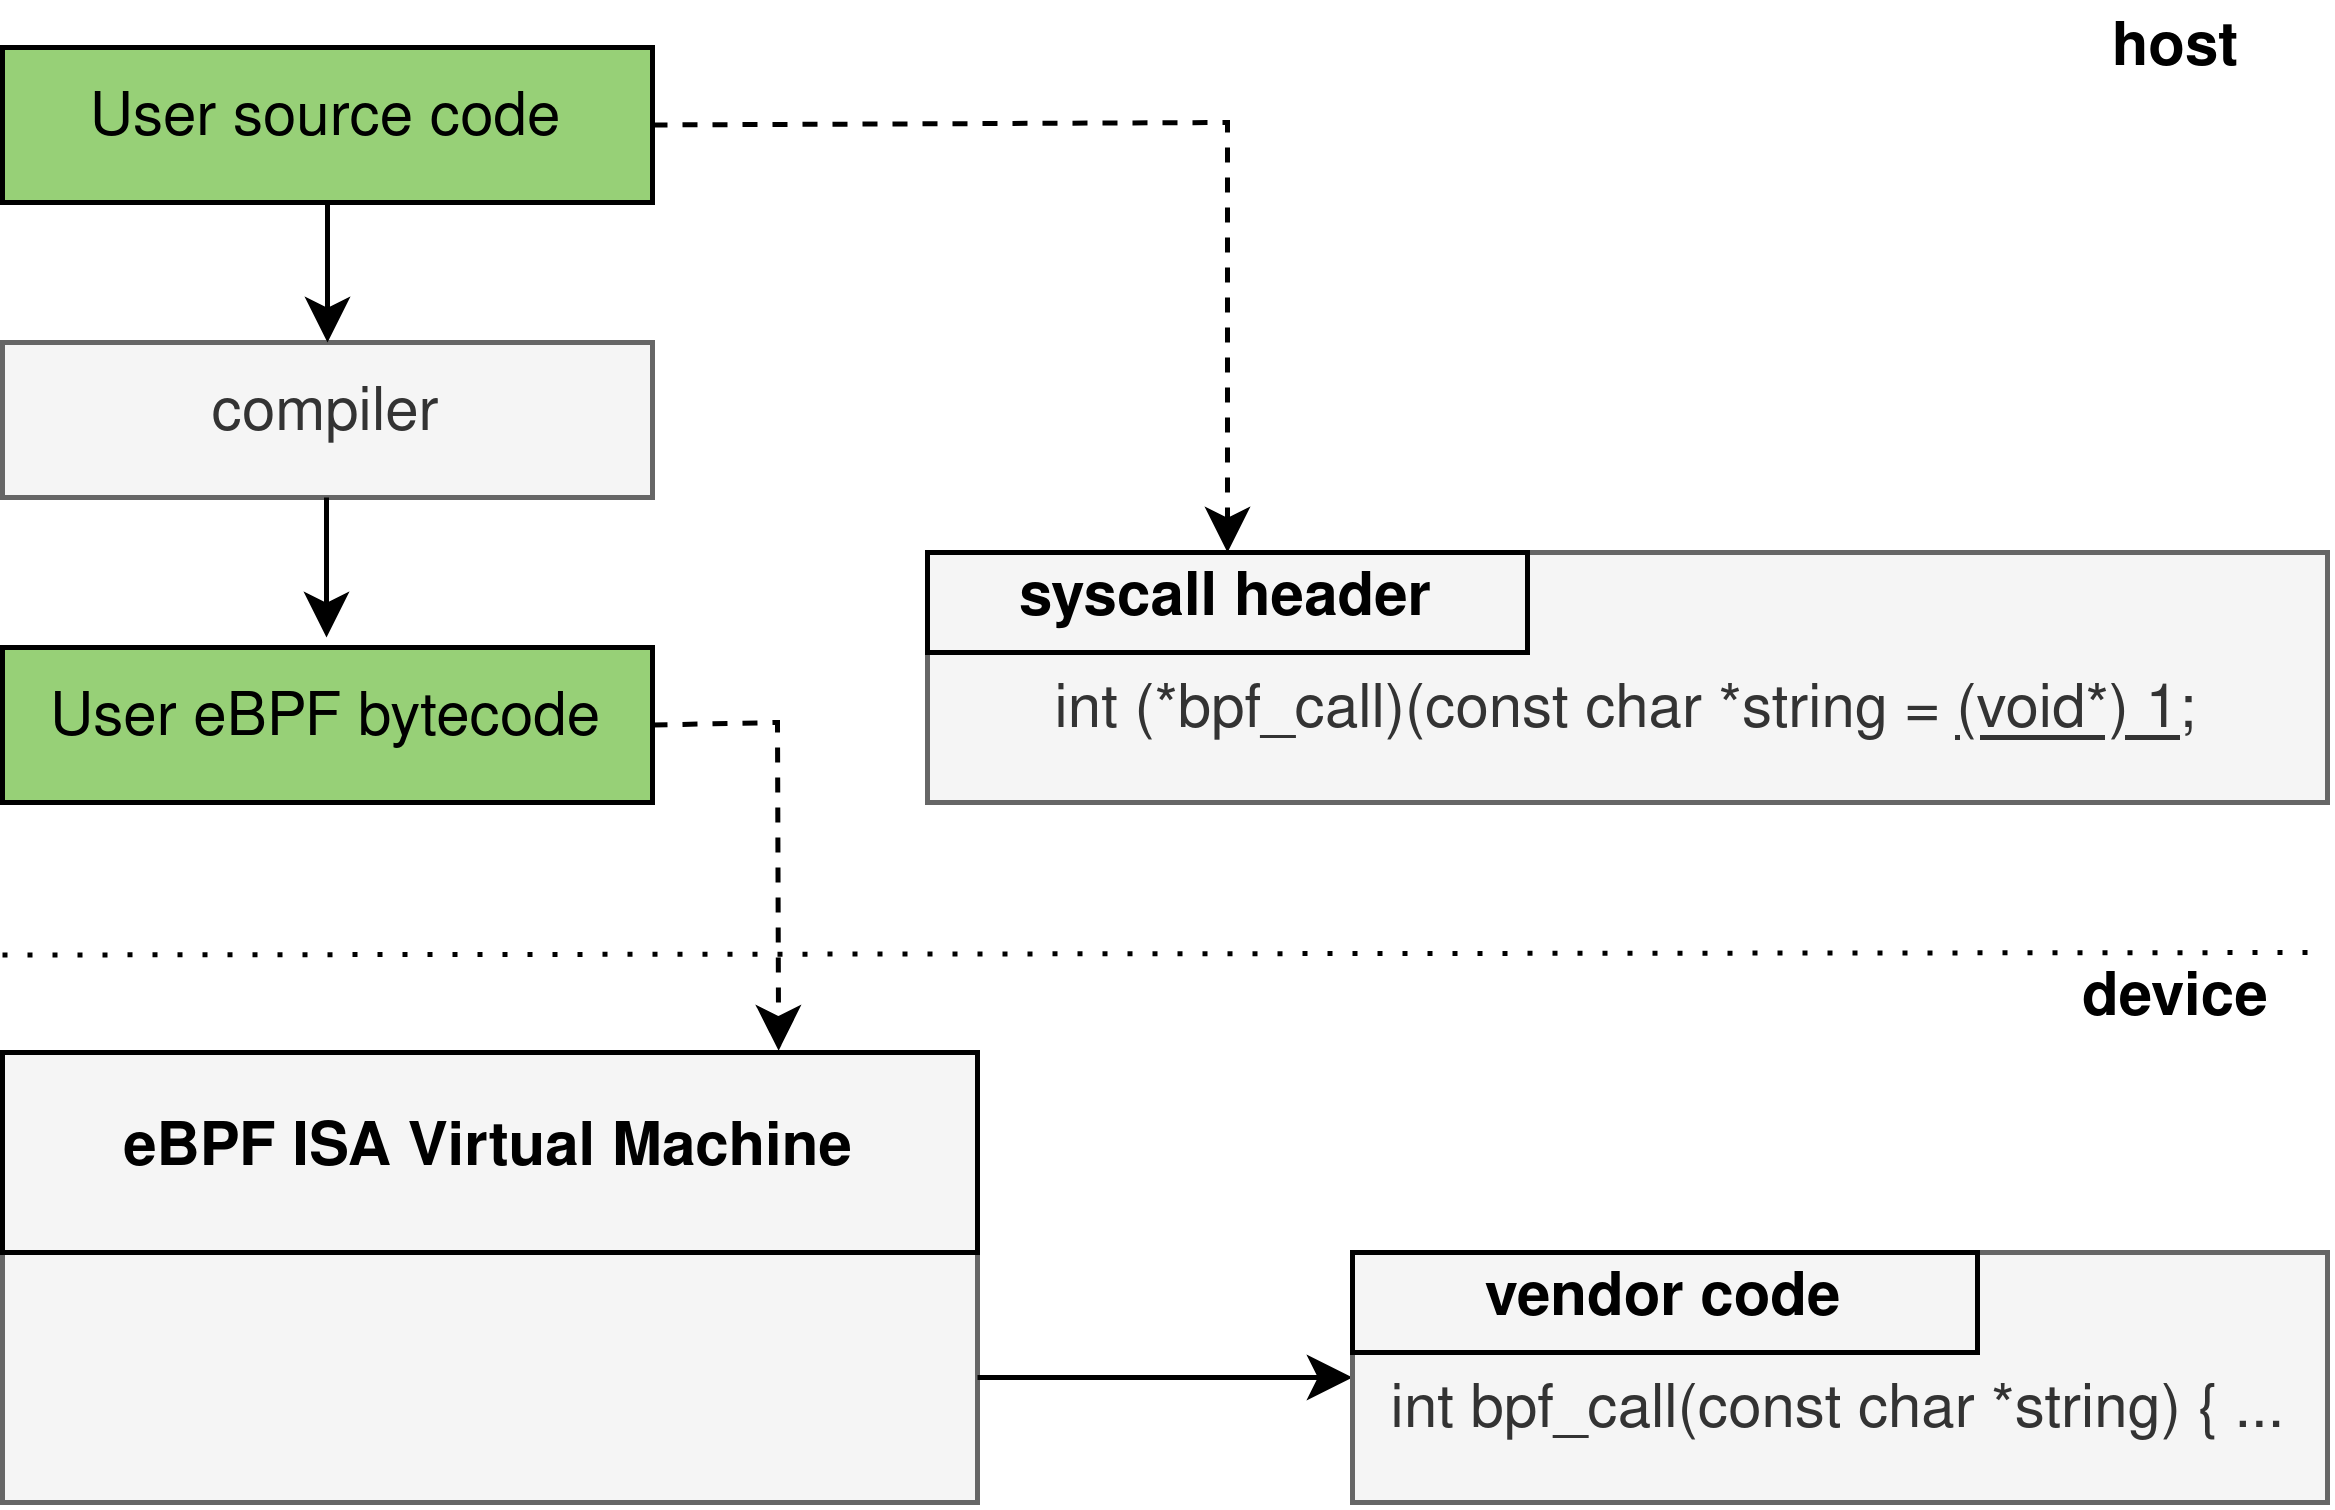
\includegraphics[width=1\textwidth]{resources/images/ubpf-medium-design.png}
            \end{figure}
            \endgroup
        \end{column}
    \end{columns}
\end{frame}
\note{
    1.5m - 15
    \begin{itemize}
        \item eBPF extensively used in the Linux kernel
        \item Used for hooks in events, receiving network packets etc
        \item Statically verified. runtime limited, on Linux
        \item eBPF essentially just an ISA, allows to define system calls
        \item ISA designed to be easily implemented by a VM.
        \item Clang supports compiling a subset of C to eBPF bytecode.
        \item Key feature, is trapped code for system call determined by VM
        \item Allows to define an ABI completely agnostic from the vendors
              implementation
        \item Using an VM allows to re-use user programs on any device
              architecture
    \end{itemize}
}

% \begin{frame}{Shannon Entropy Demo - Setup QEMU}
%         \begin{columns}
%             \begin{column}{0.42\textwidth}
%                 \footnotesize
%                 QEMU Setup
%                 \begin{itemize}
%                     \item Emulates ZNS storage device
%                     \item ~15 Gb storage requirement
%                     \begin{itemize}
%                         \item Downloads ~4.5 Gb qcow image
%                     \end{itemize}
%                     \item Re-run cmake to detect dependencies
%                 \end{itemize}
%             \end{column}
%             \begin{column}{0.58\textwidth}
%                 \begingroup
%                 \small
%                 \begin{figure}
%                     \centering
%                     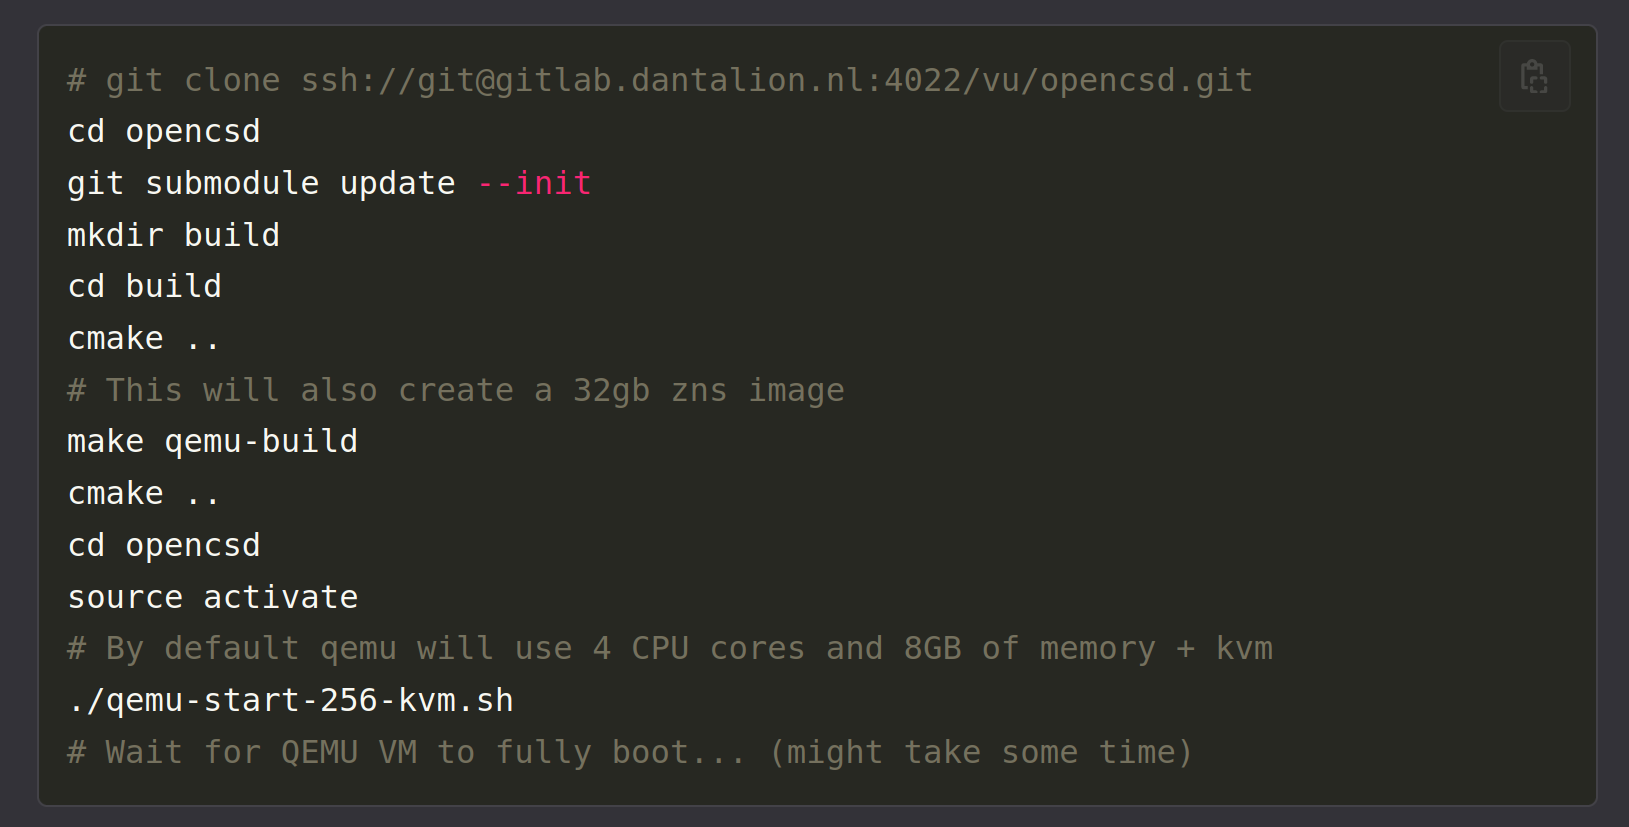
\includegraphics[width=1\textwidth]{resources/images/qemu-setup.png}
%                 \end{figure}
%                 \endgroup
%             \end{column}
%         \end{columns}
% \end{frame}
% \note{
%     1m - 15.0
%     \begin{itemize}
%         \item Please see project readme for better / more detailed instructions,
%               No need to remember these.
%         \item Image download has 30 minute time out, alternate torrent link
%               available in readme.
%         \item QEMU setup also creates 32gb zns image for non-volatile storage
%               emulation.
%         \item No longer required to compile QEMU from scratch, ZNS support used
%               to be so new it was only available on developer branch outside
%               of main QEMU repo.
%     \end{itemize}
% }
%
% \begin{frame}{Shannon Entropy Demo - Setup FluffleFS}
%         \begin{columns}
%             \begin{column}{0.40\textwidth}
%                 \footnotesize
%                 Build FluffleFS
%                 \begin{itemize}
%                     \item Login to QEMU VM
%                     \item Update included repo
%                     \item Get only necessary submodules
%                     \item Don't build QEMU inside QEMU
%                     \item Build FluffleFS filesystem
%                 \end{itemize}
%             \end{column}
%             \begin{column}{0.60\textwidth}
%                 \begingroup
%                 \small
%                 \begin{figure}
%                     \centering
%                     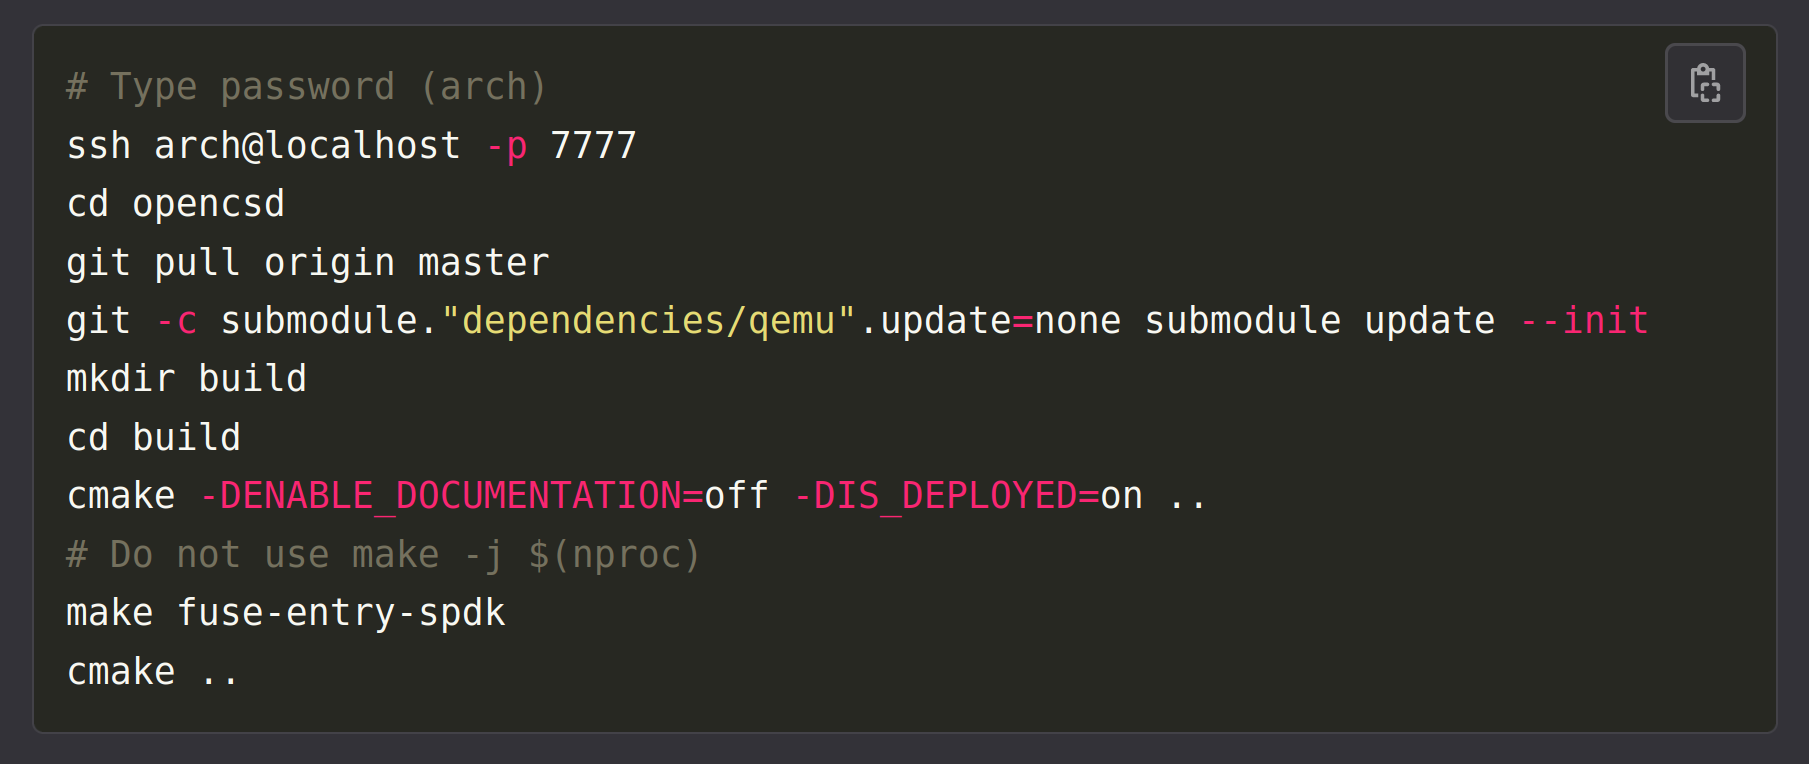
\includegraphics[width=1\textwidth]{resources/images/qemu-setup2.png}
%                 \end{figure}
%                 \endgroup
%             \end{column}
%         \end{columns}
% \end{frame}
% \note{
%     1m - 16.0
%     \begin{itemize}
%         \item \textit{-DIS\_DEPLOYED=on} disables QEMU built
%     \end{itemize}
% }

\begin{frame}{Shannon Entropy Demo}
        \begin{columns}
            \begin{column}{0.40\textwidth}
                \footnotesize
                Compute distribution of byte values
                \begin{itemize}
                    \item For project setup and install see README
                    \item Determine if file suitable for compression
                    \item
                \end{itemize}
            \end{column}
            \begin{column}{0.60\textwidth}
                \begingroup
                \small
                \begin{figure}
                    \centering
                    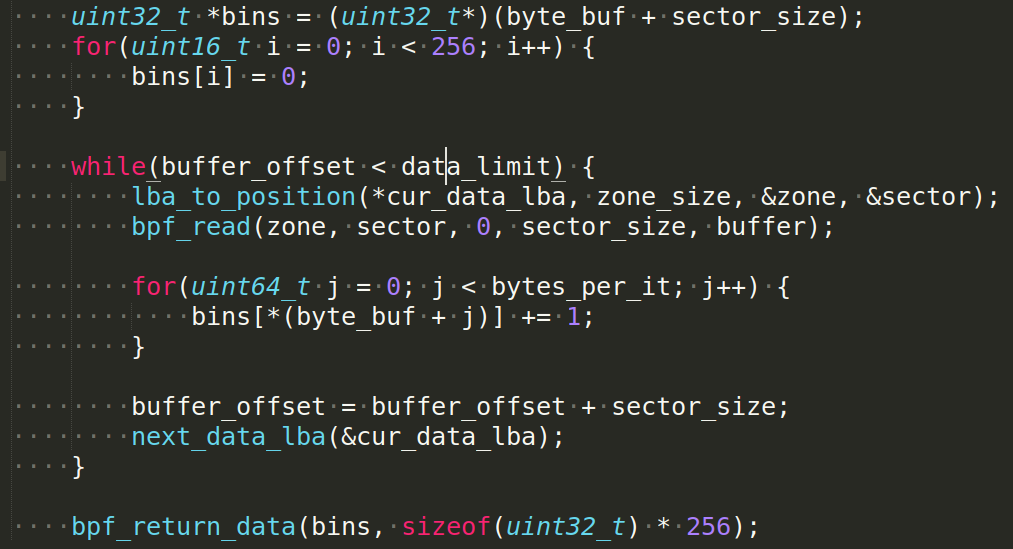
\includegraphics[width=1\textwidth]{resources/images/demo-kernel.png}
                \end{figure}
                \endgroup
            \end{column}
        \end{columns}
\end{frame}
\note{
    1m - 17.0
    \begin{itemize}
        \item Shannon Entropy determines value distribution, can be for
              bits / bytes, arbitrary size. Using granularity of memory
              interface makes most sense.
        \item
    \end{itemize}
}

\begin{frame}{Shannon Entropy Demo - Kernel}
        \begin{columns}
            \begin{column}{0.40\textwidth}
                \footnotesize
                \begin{itemize}
                    \item eBPF very small stack size
                    \item Get heap pointer, manually offset
                    \item System calls provided by eBPF
                    \item Helper functions \& data structures provided
                          by filesystem
                    \item Can we make user programs agnostic to filesystem?
                \end{itemize}
            \end{column}
            \begin{column}{0.60\textwidth}
                \begingroup
                \small
                \begin{figure}
                    \centering
                    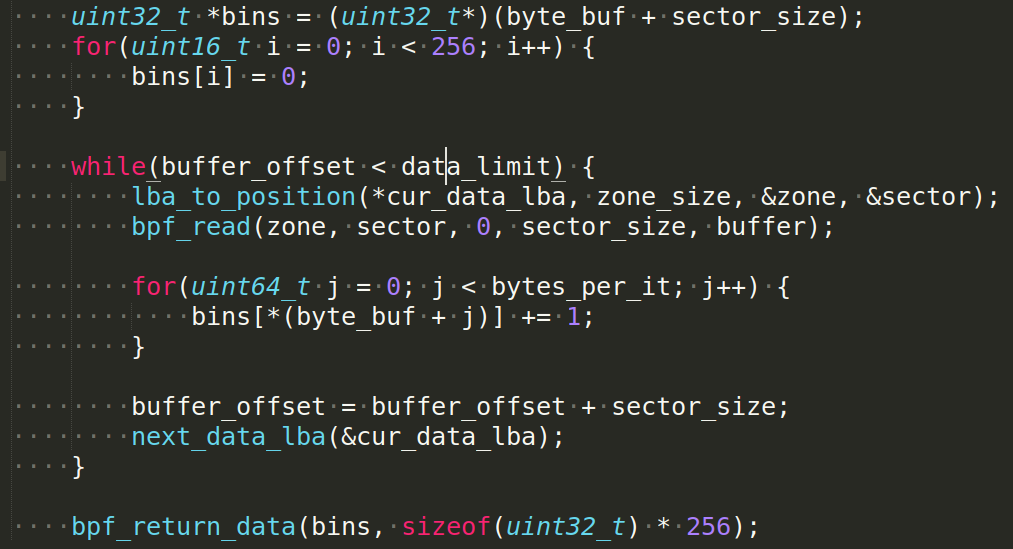
\includegraphics[width=1\textwidth]{resources/images/demo-kernel.png}
                \end{figure}
                \endgroup
            \end{column}
        \end{columns}
\end{frame}
\note{
    1m - 18.0
    \begin{itemize}
        \item Offset buffer for sector data and store histogram / bin data.
        \item Read each sector of the request and go through each byte.
        \item
    \end{itemize}
}

\begin{frame}{Shannon Entropy Demo - Execution}
    \begin{columns}
        \begin{column}{0.40\textwidth}
            \footnotesize
            How to submit I/O requests to execute kernels?
            \begin{itemize}
                \item Stride requests (FUSE page limit)
                \item Inode from kernel file as value for extended attribute
                      Key
                \item Different keys for different types of offloading
                \item Return data from \textit{os.pread} less then request
                      size.
            \end{itemize}
        \end{column}
        \begin{column}{0.60\textwidth}
            \begingroup
            \small
            \begin{figure}
                \centering
                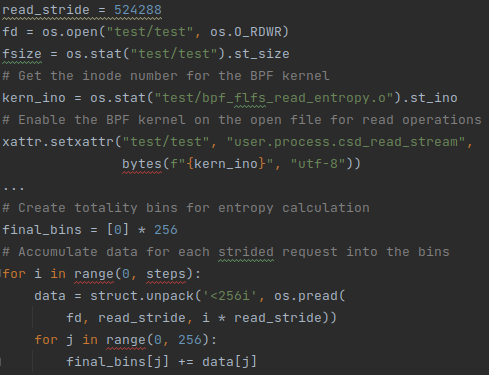
\includegraphics[width=0.85\textwidth]{resources/images/python-kernel.png}
            \end{figure}
            \endgroup
        \end{column}
    \end{columns}
\end{frame}
\note{
    1m - 19.0
    \begin{itemize}
        \item Example in Python can also easily be done in C/C++
        \item
    \end{itemize}
}

\begin{frame}{Operating Principle Details}
    \begin{columns}
        \begin{column}{0.40\textwidth}
            \footnotesize
            \begin{itemize}
                \item Stream vs Event kernels
                \item When to take snapshots?
                \begin{itemize}
                    \item Upon \textit{setxattr}
                \end{itemize}
                \item Isolate by filehandle, pid, inode?
                \begin{itemize}
                    \item By pid
                \end{itemize}
            \end{itemize}
            \textit{}
        \end{column}
        \begin{column}{0.60\textwidth}
            \begingroup
            \small
            \begin{figure}
                \centering
                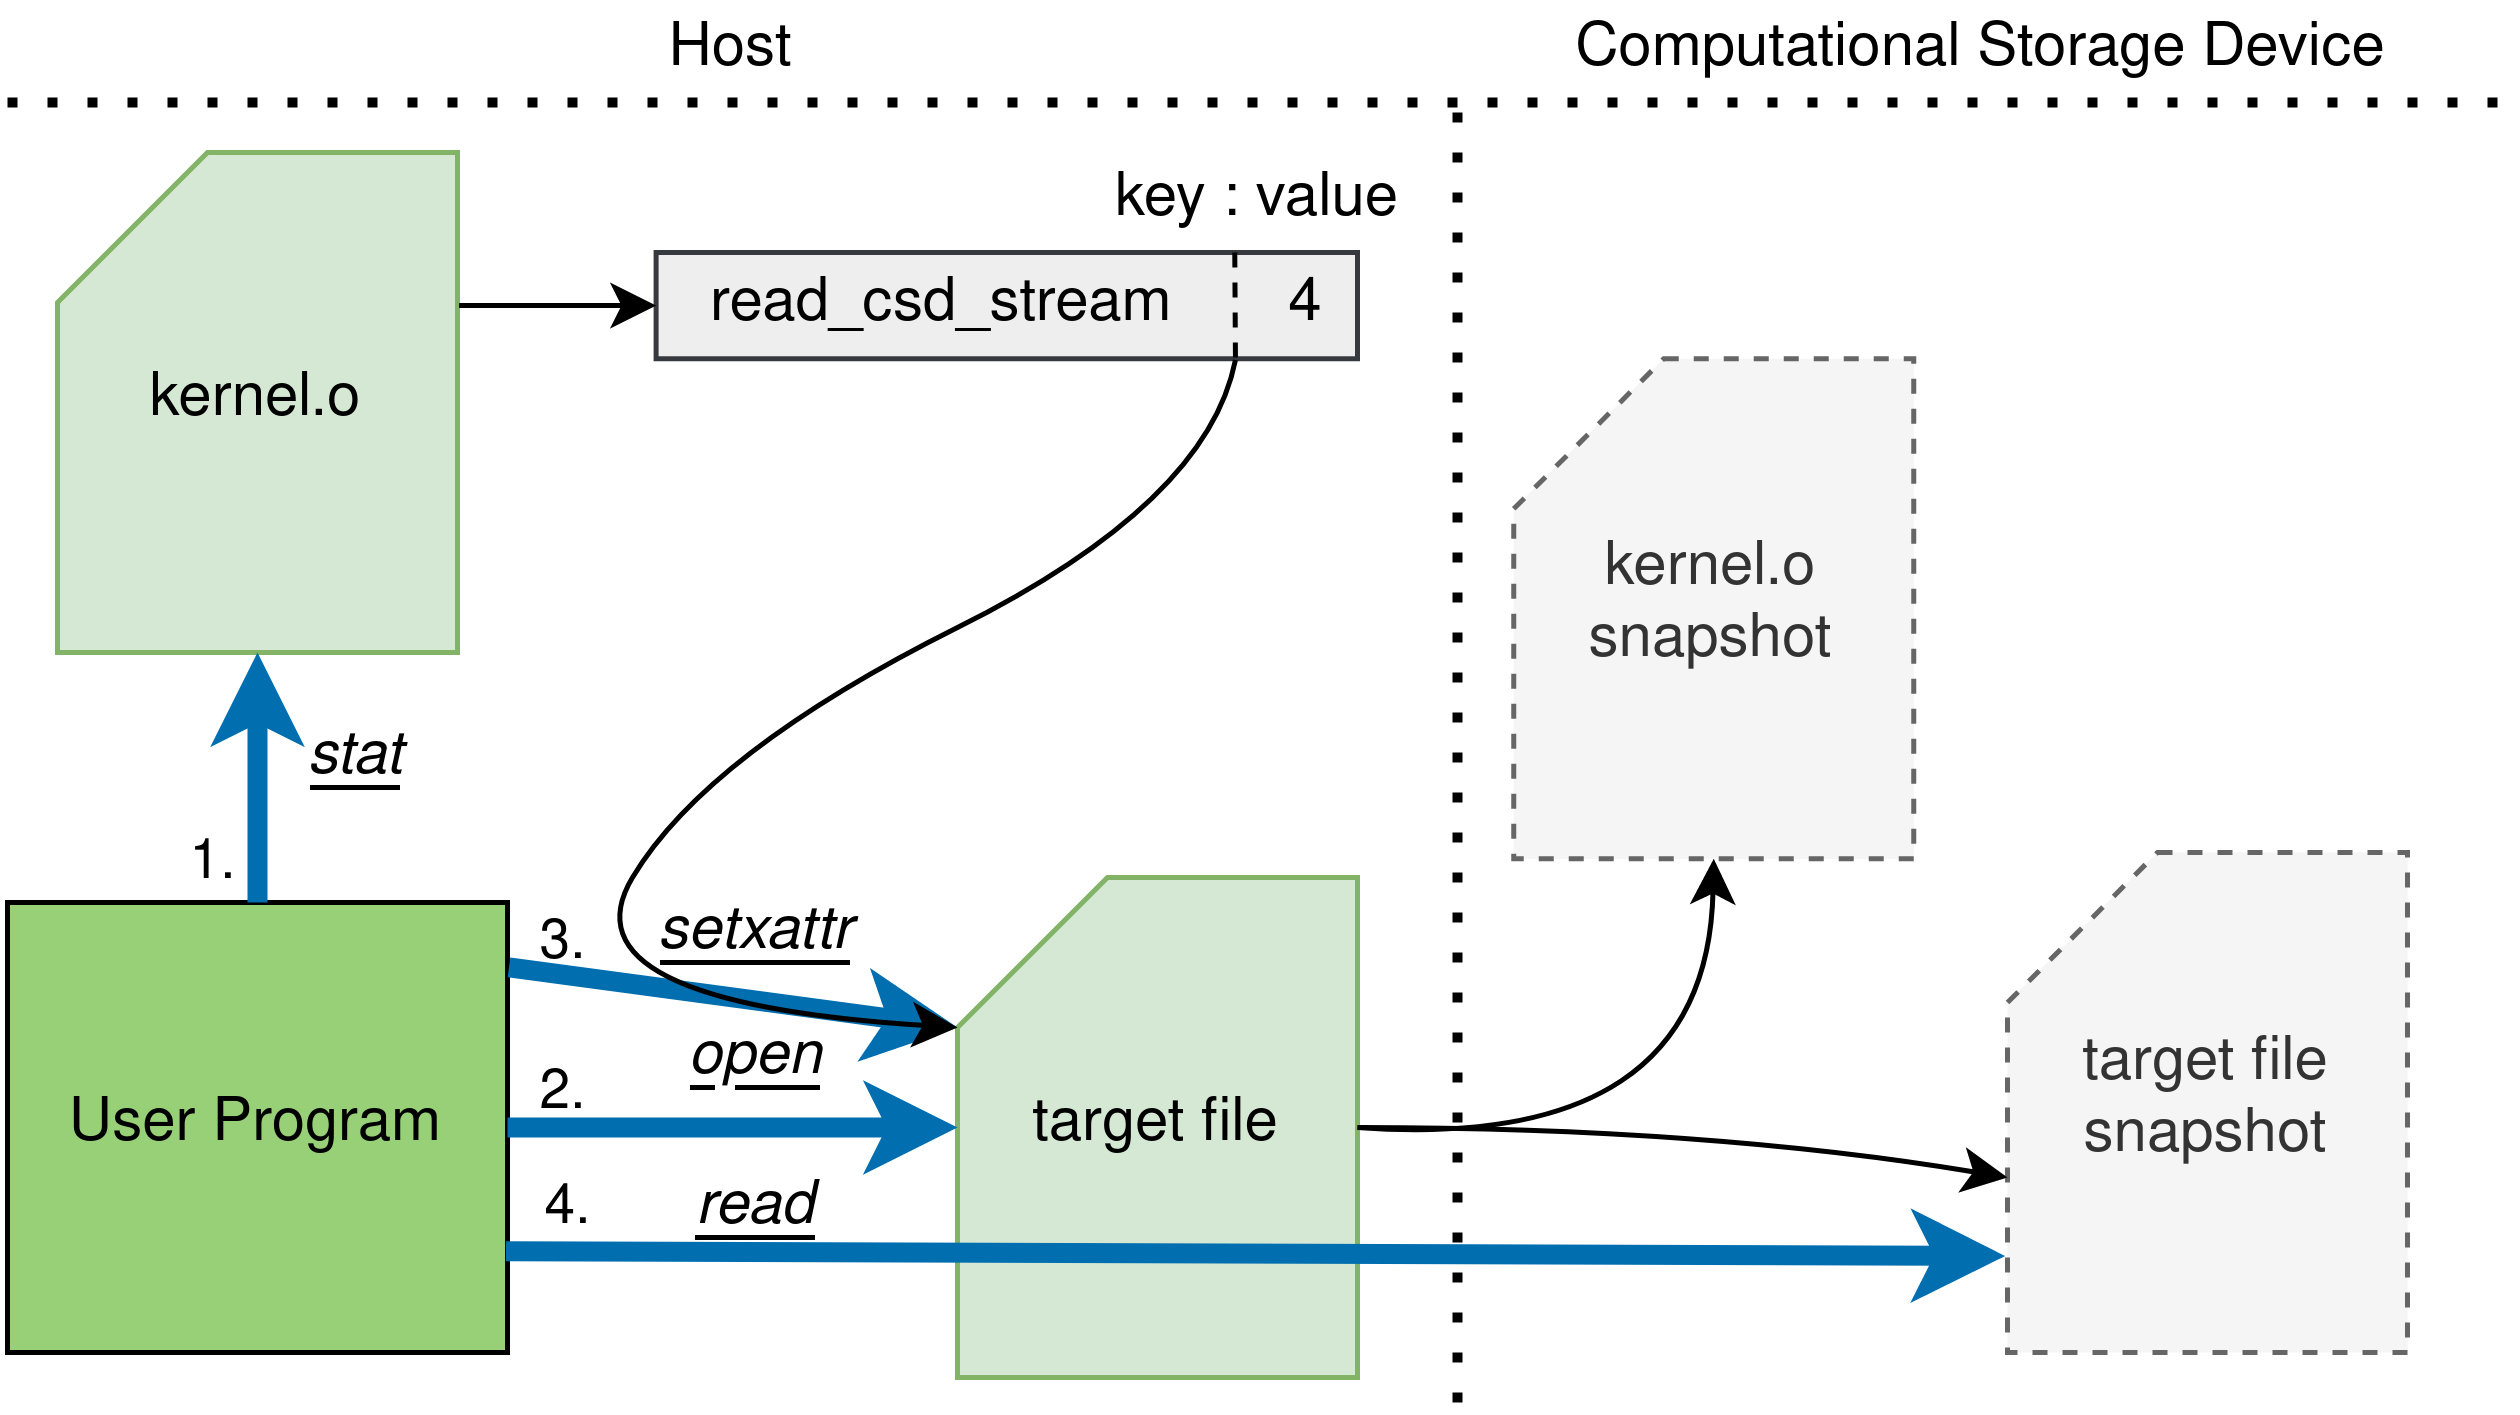
\includegraphics[width=1\textwidth]{resources/images/offloading.png}
            \end{figure}
            \endgroup
        \end{column}
    \end{columns}
\end{frame}
\note{
    1m - 20.0
    \begin{itemize}
        \item We distinguish between stream kernels and event kernels
        \item Stream: Happens in-place of the regular I/O request
        \item Event: Happens after the regular I/O request completes normally
        \item Kernel and target file have to be on the same filesystem
    \end{itemize}
}

\begin{frame}{Limitations and Considerations}
    \begin{columns}
        \begin{column}{0.50\textwidth}
            \footnotesize
            \begin{itemize}
                \item Filesystem (FluffleFS) is \textbf{solely} proof of
                      concept!
                \item eBPF endian conversions and datastructure layouts
                \item Runtime execution of compute kernels \textbf{not}
                      cycle accurate
                \item Only, \textit{read stream} kernel fully supported
                \item File system agnostic kernels
            \end{itemize}
            \textit{}
        \end{column}
        \begin{column}{0.50\textwidth}
            \begingroup
            \small
            \begin{figure}
                \centering
                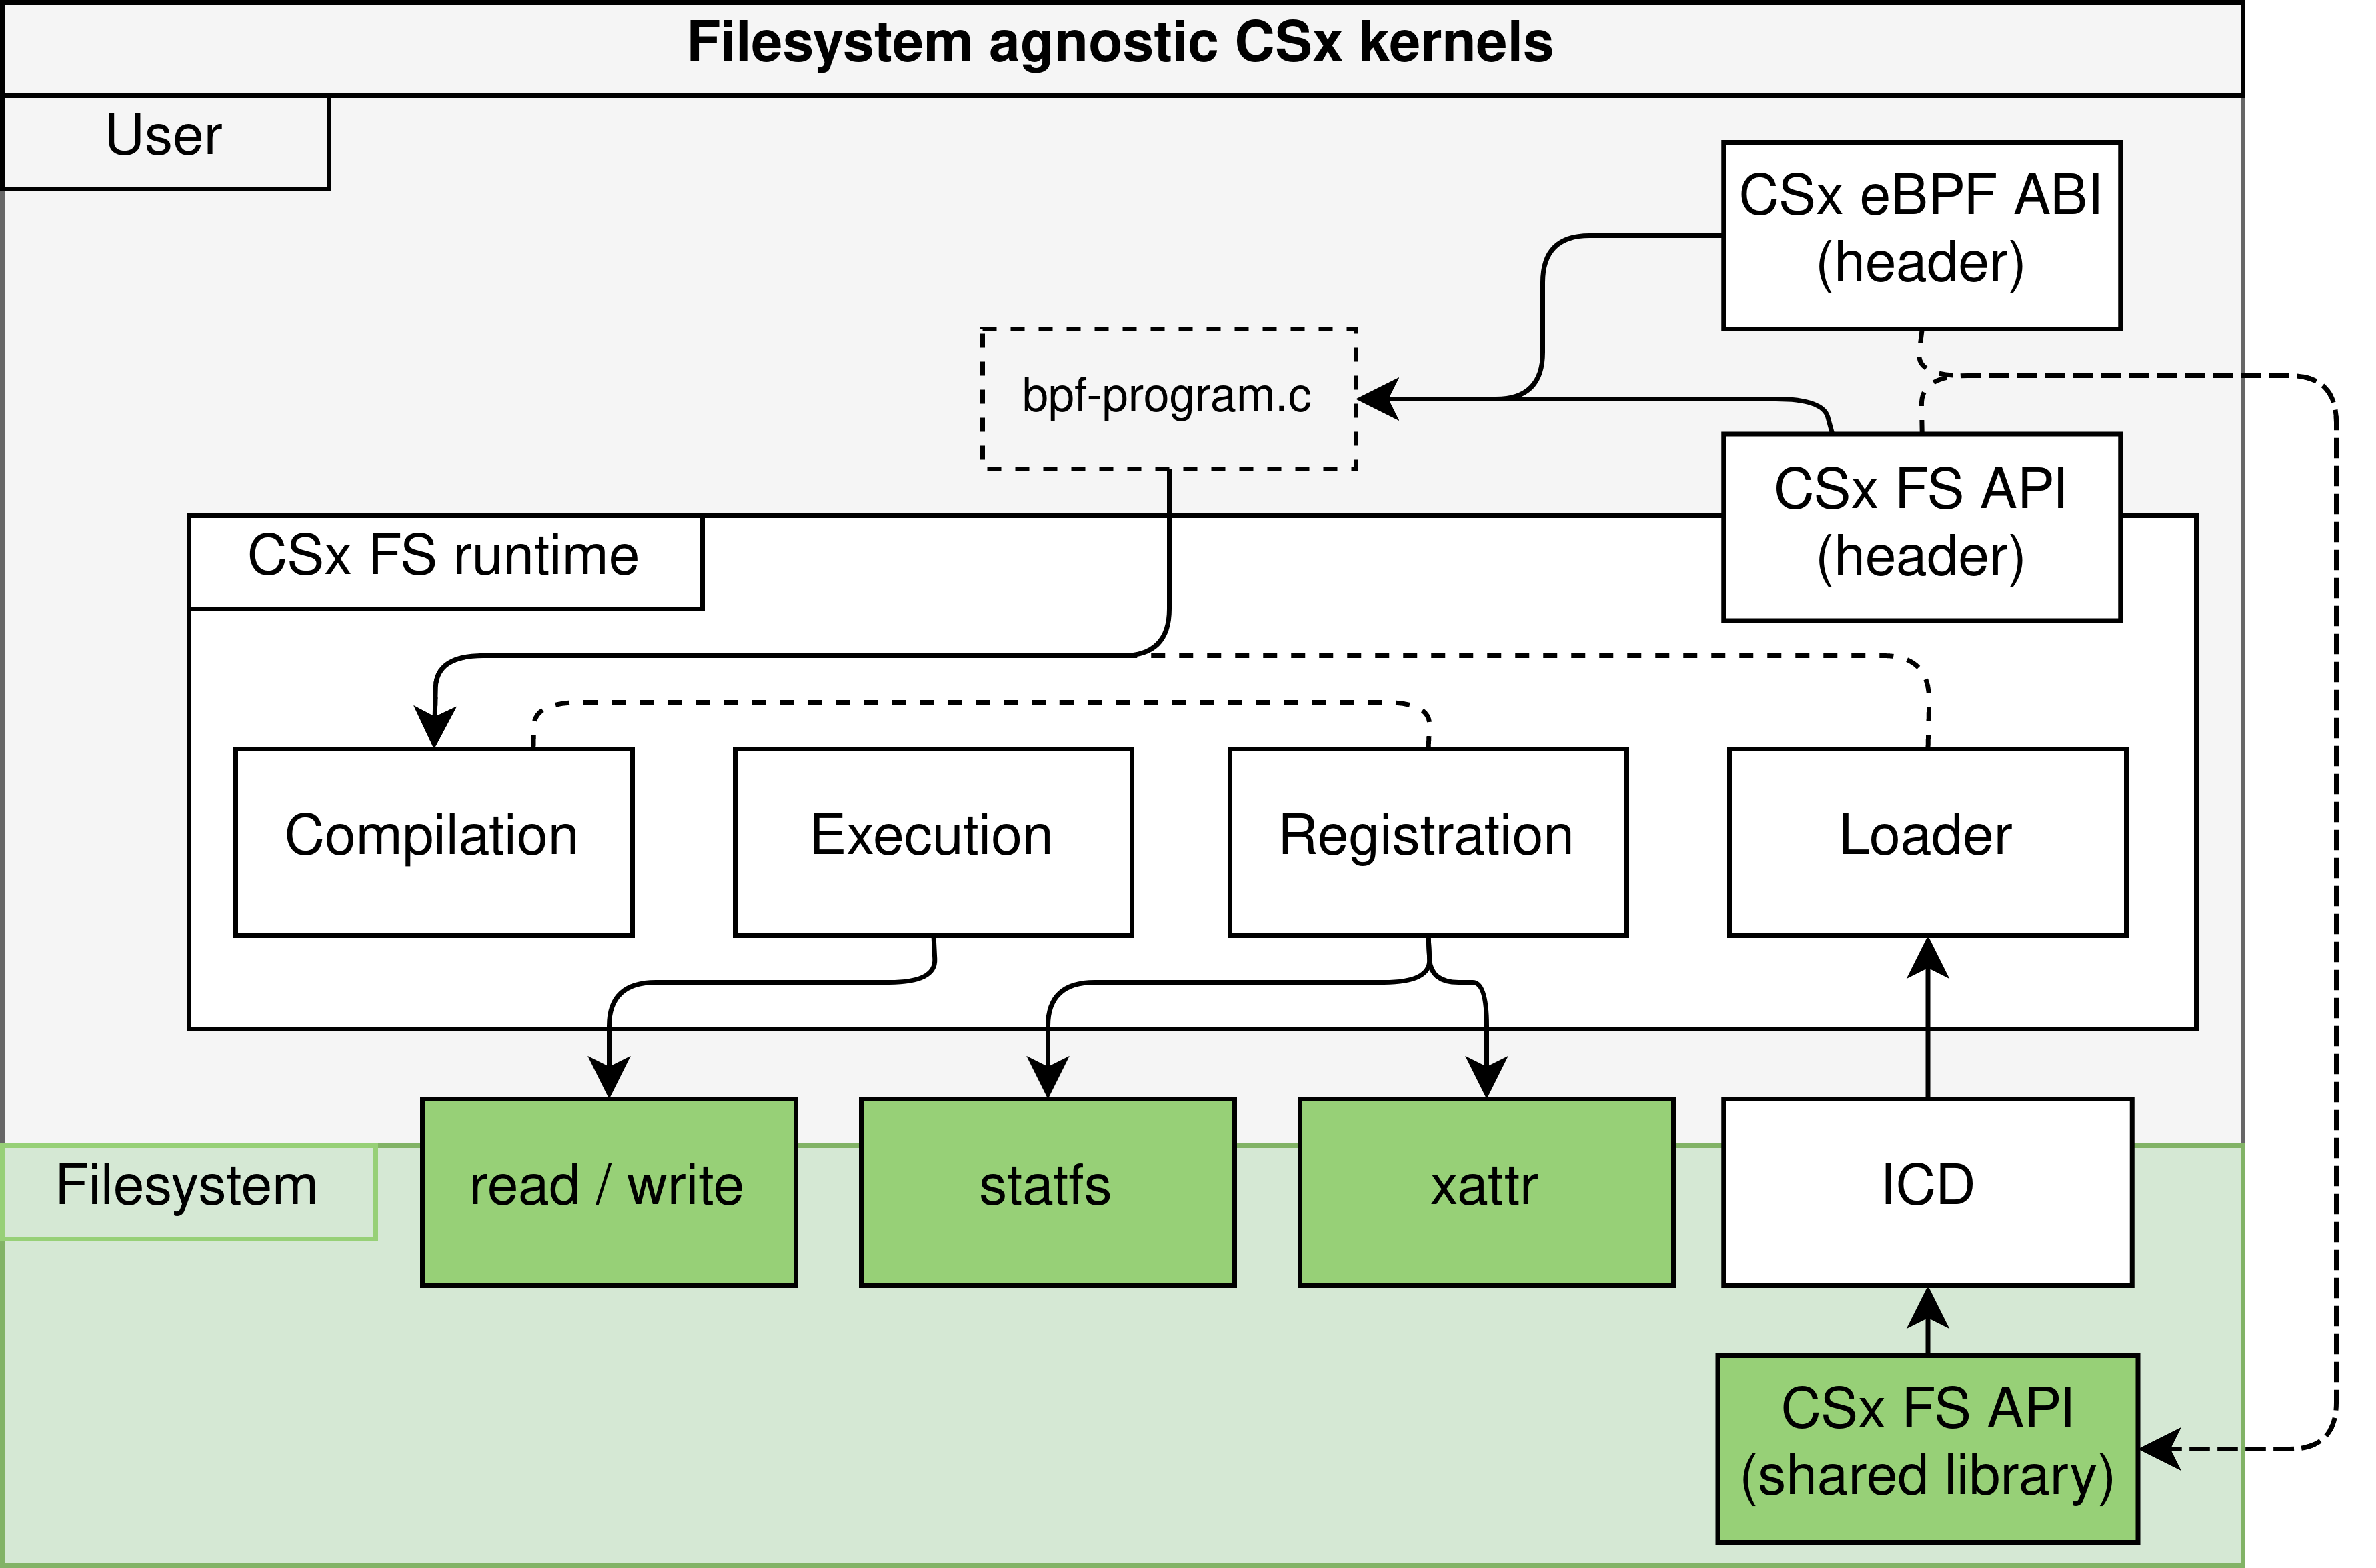
\includegraphics[width=1\textwidth]{resources/images/csx-fs-agnostic.png}
            \end{figure}
            \endgroup
        \end{column}
    \end{columns}
\end{frame}
\note{
    1m - 21.0
    \begin{itemize}
        \item Filesystem, no gc, no deletion, no space reclaiming
        \item My first filesystem, should be redesigned from zero
        \item eBPF kernels run on the host CPU, no cycle accurate
              representation of SSD microcontrollers.
    \end{itemize}
}

% page 11
% All software and data to this project is open source, this includes scripts to
% perform measurements, raw measurement data, scripts to generate graphs and
% even source files to this very presentation. We heavily encourage anyone to
% try it today, there is an extensive readme which includes a video on how to
% setup the project and the source code is extensively documented as well.
% I can not stress enough how important I think this sort of openenness is
% for the reproducability in computer science research. In highly encourage
% everyone to re-evelauate what they are doing to ensure others can reproduce
% their works as well. Thanks you for listening.
\begin{frame}{Further Reading}
	\begingroup
	\small Try it today! \underline{\url{https://github.com/Dantali0n/OpenCSD}}
	\begin{itemize}
		\item OpenCSD: Log-Structured Filesystem enabled Computational
		Storage Device platform - https://tinyurl.com/opencsd-thesis
		\item ZCSD: a Computational Storage Device over Zoned Namespaces (ZNS)
			SSDs - https://arxiv.org/abs/2112.00142
		\item Past, Present and Future of Computational Storage: A Survey
			- https://arxiv.org/abs/2112.09691
	\end{itemize}
	\endgroup
\end{frame}
\note{
    1m - 22.0
    \begin{itemize}
        \item Completely omitted details about filesystem and datastructures,
              see thesis work.
        \item No details about performance see thesis or earlier ZCSD work.
        \item Detailed history of computation storage see survey
        \item Above all, try the prototype today. Go through the readme,
              write your own kernels
    \end{itemize}
}

\end{document}